\documentclass[11pt,a4paper]{article}

% ----------------------------------------------------------------------------- pacotes
\usepackage[T1]{fontenc}
\usepackage[utf8]{inputenc}
\usepackage{lmodern}
\usepackage[english,brazilian]{babel}
\usepackage[a4paper,margin=2.5cm]{geometry}
\usepackage{amsmath,amssymb}
\usepackage{graphicx}
\usepackage{booktabs}
\usepackage{siunitx}
\sisetup{output-decimal-marker={,}, group-separator={.}, group-minimum-digits=4,
         input-symbols={<>}, retain-explicit-plus}
\usepackage{csquotes}
\usepackage[backend=biber,style=authoryear,maxcitenames=2,maxbibnames=10,uniquelist=false,
            uniquename=false,doi=true,url=false,isbn=false,dashed=false]{biblatex}
\addbibresource{refs.bib}
\usepackage{xcolor}
\usepackage[colorlinks=true,linkcolor=blue!50!black,citecolor=blue!50!black,urlcolor=blue!50!black]{hyperref}
\usepackage[capitalise,noabbrev]{cleveref}
\crefname{figure}{Figura}{Figuras}
\crefname{table}{Tabela}{Tabelas}
\crefname{section}{Seção}{Seções}
\crefname{equation}{Equação}{Equações}
\newcommand{\crefpairconjunction}{ e }
\newcommand{\crefmiddleconjunction}{, }
\newcommand{\creflastconjunction}{ e }
\newcommand{\crefrangeconjunction}{ a }
\usepackage{caption}
\captionsetup{font=small,labelfont=bf}
\setlength{\emergencystretch}{2em}   % evita estouro de margem em linhas com muitos números

% Gerado automaticamente por scripts/paper.jl — NÃO EDITAR À MÃO.
% 2026-10-17 09:36 | 949 macros
\newcommand{\AICChuvaDegrau}{\num{481.4}}
\newcommand{\AICChuvaLinear}{\num{476.1}}
\newcommand{\AnoCorteValidacao}{2005/06}
\newcommand{\AnoDegrauChuva}{2009/10}
\newcommand{\AnoMinimo}{2016/17}
\newcommand{\AnosCobertosSPI}{\num{41}}
\newcommand{\AnosFCASete}{1981/82, 2021/22, 2023/24}
\newcommand{\AnosSemEstacao}{1975/76, 1992/93, 1997/98, 2011/12, 2012/13, 2015/16, 2016/17}
\newcommand{\BTmaxDegrau}{\num{0.23}}
\newcommand{\BTmaxDegrauICinf}{\num{0.06}}
\newcommand{\BTmaxDegrauICsup}{\num{0.41}}
\newcommand{\BayesNSEfeito}{\num{-12.1}}
\newcommand{\BayesNSEfeitoICinf}{\num{-17.5}}
\newcommand{\BayesNSEfeitoICsup}{\num{-6.5}}
\newcommand{\CentroideMedio}{07/02}
\newcommand{\ChuvaDozeTreze}{\num{151.3}}
\newcommand{\ChuvaDozeTrezeComb}{\num{103.2}}
\newcommand{\ChuvaJanNormal}{\num{85}}
\newcommand{\ChuvaJanNormalOficial}{\num{83.5}}
\newcommand{\ChuvaMarNormal}{\num{84}}
\newcommand{\ChuvaMarNormalOficial}{\num{83.6}}
\newcommand{\ChuvaMarSeisUmOficial}{\num{136}}
\newcommand{\ChuvaMinima}{\num{134.9}}
\newcommand{\ConcMedia}{\num{0.65}}
\newcommand{\CorteSeco}{\num{392}}
\newcommand{\DPChuvaValidos}{\num{183}}
\newcommand{\DegrauTmax}{\num{0.14}}
\newcommand{\DifIniTmaxCabrobo}{\num{5.1}}
\newcommand{\DifIniTmaxRemanso}{\num{3.2}}
\newcommand{\DifIniTminCabrobo}{\num{0.9}}
\newcommand{\DifIniTminRemanso}{\num{0.4}}
\newcommand{\DifMediaTmax}{\num{0.08}}
\newcommand{\DifMediaTmin}{\num{-0.31}}
\newcommand{\DifNormalChuvaMensalMax}{\num{1.8}}
\newcommand{\DifNormalTempMax}{\num{0.05}}
\newcommand{\DifPersistencia}{\num{0.20}}
\newcommand{\DifPersistenciaICinf}{\num{-0.09}}
\newcommand{\DifPersistenciaICsup}{\num{0.47}}
\newcommand{\DifPosTmaxCabrobo}{\num{-0.1}}
\newcommand{\DifPosTmaxRemanso}{\num{0.5}}
\newcommand{\DifPosTminCabrobo}{\num{0.2}}
\newcommand{\DifPosTminRemanso}{\num{-0.2}}
\newcommand{\DistCavalos}{\num{23}}
\newcommand{\DistJuazeiro}{\num{3}}
\newcommand{\DistJunco}{\num{33}}
\newcommand{\DistLagoaBoi}{\num{37}}
\newcommand{\DistLagoaGrande}{\num{51}}
\newcommand{\DistRejeitadasAD}{lognormal}
\newcommand{\DuracaoMediana}{\num{135}}
\newcommand{\DuracaoSeca}{\num{2.0}}
\newcommand{\DuracaoSecaICinf}{\num{1.4}}
\newcommand{\DuracaoSecaICsup}{\num{3.7}}
\newcommand{\ESSMin}{\num{2539}}
\newcommand{\ESSMinNS}{\num{2825}}
\newcommand{\EfeitoFormaGamma}{\num{-24.8}}
\newcommand{\EfeitoFormaLogNormal}{\num{17.0}}
\newcommand{\EfeitoFormaNormal}{\num{-0.6}}
\newcommand{\EfeitoFormaWeibull}{\num{-11.4}}
\newcommand{\EspEumEstGamma}{\num{0.02}}
\newcommand{\EspEumEstMedia}{\num{0.11}}
\newcommand{\EspEumNSGamma}{\num{0.07}}
\newcommand{\EspEumNSMedia}{\num{0.60}}
\newcommand{\EspEumNSNormal}{\num{0.86}}
\newcommand{\EspPdezEstGamma}{\num{1.98}}
\newcommand{\EspPdezEstMedia}{\num{2.03}}
\newcommand{\EspPdezNSGamma}{\num{5.60}}
\newcommand{\EspPdezNSMedia}{\num{5.85}}
\newcommand{\EspPdezNSNormal}{\num{5.74}}
\newcommand{\EvRefDuracao}{\num{21}}
\newcommand{\EvRefFim}{11/2013}
\newcommand{\EvRefInicio}{03/2012}
\newcommand{\EvRefIntensidade}{\num{1.91}}
\newcommand{\EvRefPico}{\num{-2.95}}
\newcommand{\EvRefRankSeveridade}{\num{1}}
\newcommand{\EvRefSeveridade}{\num{40.1}}
\newcommand{\FCAdoiszerodoistresdoisquatro}{\num{5.4}}
\newcommand{\FCAdoiszerodoisumdoisdois}{\num{7.0}}
\newcommand{\FCAumnoveoitoumoitodois}{\num{7.2}}
\newcommand{\FimMediano}{14/04}
\newcommand{\FracNovAbr}{\num{91}}
\newcommand{\GammaEscala}{\num{79.1}}
\newcommand{\GammaForma}{\num{6.08}}
\newcommand{\GammaPAD}{\num{0.15}}
\newcommand{\GammaPesoAkaike}{\num{0.13}}
\newcommand{\InicioMediano}{23/11}
\newcommand{\LimiarPdez}{\num{345}}
\newcommand{\MDTCDD}{\num{12.2}}
\newcommand{\MDTCWD}{\num{0.7}}
\newcommand{\MDTCentroide}{\num{6.3}}
\newcommand{\MDTConc}{\num{0.041}}
\newcommand{\MDTDTR}{\num{0.17}}
\newcommand{\MDTDuracao}{\num{12.1}}
\newcommand{\MDTFim}{\num{6.0}}
\newcommand{\MDTFracNovAbr}{\num{0.022}}
\newcommand{\MDTInicio}{\num{12.1}}
\newcommand{\MDTRnovecincop}{\num{24}}
\newcommand{\MDTRummm}{\num{3.3}}
\newcommand{\MDTRxumday}{\num{7.7}}
\newcommand{\MDTSDII}{\num{0.74}}
\newcommand{\MDTSI}{\num{0.045}}
\newcommand{\MDTTNn}{\num{0.35}}
\newcommand{\MDTTNumzerop}{\num{3.4}}
\newcommand{\MDTTXnovezerop}{\num{1.3}}
\newcommand{\MDTTXx}{\num{0.25}}
\newcommand{\MDTTmax}{\num{0.14}}
\newcommand{\MDTTmed}{\num{0.16}}
\newcommand{\MDTTmin}{\num{0.11}}
\newcommand{\MDTUR}{\num{1.2}}
\newcommand{\MDTVento}{\num{0.08}}
\newcommand{\MediaChuvaAteDoisMilNove}{\num{536}}
\newcommand{\MediaChuvaValidos}{\num{481}}
\newcommand{\MelhorAIC}{Weibull}
\newcommand{\MelhorAICNS}{normal}
\newcommand{\MelhorAICNSForma}{fixa}
\newcommand{\MesDifNormalChuva}{janeiro}
\newcommand{\MesMaisChuvoso}{janeiro}
\newcommand{\MinComumAna}{\num{30}}
\newcommand{\NAnaAntesDepoisSig}{\num{1}}
\newcommand{\NAnaNeg}{\num{5}}
\newcommand{\NAnaNegSig}{\num{4}}
\newcommand{\NAnaQSig}{\num{2}}
\newcommand{\NBootNSMedia}{\num{2000}}
\newcommand{\NCDD}{\num{46}}
\newcommand{\NCWD}{\num{47}}
\newcommand{\NChuvaAteDezOnze}{\num{37}}
\newcommand{\NChuvaAteDoisMilNove}{\num{35}}
\newcommand{\NChuvaDesdeSetentaUm}{\num{44}}
\newcommand{\NChuvaFCASete}{\num{50}}
\newcommand{\NChuvaSemSeca}{\num{41}}
\newcommand{\NComumCavalos}{\num{47}}
\newcommand{\NComumJuazeiro}{\num{35}}
\newcommand{\NComumJunco}{\num{39}}
\newcommand{\NComumLagoaBoi}{\num{40}}
\newcommand{\NComumLagoaGrande}{\num{42}}
\newcommand{\NDTR}{\num{42}}
\newcommand{\NDistRejeitadasAD}{\num{1}}
\newcommand{\NFaseNeutro}{\num{17}}
\newcommand{\NFaseNeutroDet}{\num{17}}
\newcommand{\NFaseNina}{\num{16}}
\newcommand{\NFaseNinaDet}{\num{16}}
\newcommand{\NFaseNino}{\num{14}}
\newcommand{\NFaseNinoDet}{\num{14}}
\newcommand{\NNN}{\num{19}}
\newcommand{\NNS}{\num{8}}
\newcommand{\NPostosAna}{\num{5}}
\newcommand{\NPostosAnaCandidatos}{\num{11}}
\newcommand{\NRnovecincop}{\num{47}}
\newcommand{\NRummm}{\num{47}}
\newcommand{\NRxumday}{\num{47}}
\newcommand{\NSDII}{\num{47}}
\newcommand{\NSFCASeteEfeito}{\num{-8.8}}
\newcommand{\NSN}{\num{8}}
\newcommand{\NSOniDAIC}{\num{0.3}}
\newcommand{\NSOniEfeito}{\num{-8.0}}
\newcommand{\NSOniP}{\ensuremath{=}\,\num{0.20}}
\newcommand{\NSOniPVal}{\num{0.20}}
\newcommand{\NSRegionalEfeito}{\num{-8.3}}
\newcommand{\NSS}{\num{8}}
\newcommand{\NSTempoDAIC}{\num{-13.2}}
\newcommand{\NSTempoEfeito}{\num{-12.4}}
\newcommand{\NSTempoP}{\ensuremath{<}\,\num{0.001}}
\newcommand{\NSTempoPVal}{\num{< 0.001}}
\newcommand{\NSecosNeutro}{\num{3}}
\newcommand{\NSecosNeutroDet}{\num{5}}
\newcommand{\NSecosNina}{\num{5}}
\newcommand{\NSecosNinaDet}{\num{3}}
\newcommand{\NSecosNino}{\num{8}}
\newcommand{\NSecosNinoDet}{\num{4}}
\newcommand{\NTNn}{\num{46}}
\newcommand{\NTNumzerop}{\num{46}}
\newcommand{\NTXnovezerop}{\num{47}}
\newcommand{\NTXx}{\num{47}}
\newcommand{\NTeste}{\num{15}}
\newcommand{\NTmax}{\num{47}}
\newcommand{\NTmed}{\num{42}}
\newcommand{\NTmin}{\num{46}}
\newcommand{\NTreino}{\num{32}}
\newcommand{\NUR}{\num{44}}
\newcommand{\NVento}{\num{34}}
\newcommand{\NanosAteDozeTreze}{\num{2}}
\newcommand{\NanosCurto}{\num{18}}
\newcommand{\NanosFCASete}{\num{50}}
\newcommand{\NanosHidro}{\num{65}}
\newcommand{\NanosQ}{\num{43}}
\newcommand{\NanosSemEstacao}{\num{7}}
\newcommand{\NanosValidos}{\num{47}}
\newcommand{\NeventosSPI}{\num{6}}
\newcommand{\NormalChuva}{\num{419}}
\newcommand{\NormalOficialChuva}{\num{419}}
\newcommand{\NormalOficialChuvaOitoUm}{\num{483}}
\newcommand{\NormalOficialChuvaSeisUm}{\num{577}}
\newcommand{\Npares}{\num{4}}
\newcommand{\NparesQuebraSig}{\num{0}}
\newcommand{\NquebrasTemp}{\num{2}}
\newcommand{\NtendSig}{\num{11}}
\newcommand{\NtendTotal}{\num{16}}
\newcommand{\NtestesTemp}{\num{4}}
\newcommand{\NtransicoesMarkov}{\num{43}}
\newcommand{\NvizinhasTendNeg}{\num{4}}
\newcommand{\NvizinhasTendSig}{\num{0}}
\newcommand{\NvizinhasUsadas}{\num{4}}
\newcommand{\ORSemEstacao}{\num{1.47}}
\newcommand{\ORSemEstacaoICinf}{\num{0.83}}
\newcommand{\ORSemEstacaoICsup}{\num{2.60}}
\newcommand{\ObsEum}{\num{2}}
\newcommand{\ObsPdez}{\num{7}}
\newcommand{\PAntesDepoisAnaCavalos}{\ensuremath{=}\,\num{0.84}}
\newcommand{\PAntesDepoisAnaCavalosVal}{\num{0.84}}
\newcommand{\PAntesDepoisAnaJuazeiro}{\ensuremath{=}\,\num{0.16}}
\newcommand{\PAntesDepoisAnaJuazeiroVal}{\num{0.16}}
\newcommand{\PAntesDepoisAnaJunco}{\ensuremath{=}\,\num{0.003}}
\newcommand{\PAntesDepoisAnaJuncoVal}{\num{0.003}}
\newcommand{\PAntesDepoisAnaLagoaBoi}{\ensuremath{=}\,\num{0.53}}
\newcommand{\PAntesDepoisAnaLagoaBoiVal}{\num{0.53}}
\newcommand{\PAntesDepoisAnaLagoaGrande}{\ensuremath{=}\,\num{0.47}}
\newcommand{\PAntesDepoisAnaLagoaGrandeVal}{\num{0.47}}
\newcommand{\PDozeTreze}{\num{0.012}}
\newcommand{\PFisher}{\ensuremath{=}\,\num{0.31}}
\newcommand{\PFisherVal}{\num{0.31}}
\newcommand{\PFormaVarGamma}{\ensuremath{=}\,\num{0.034}}
\newcommand{\PFormaVarGammaVal}{\num{0.034}}
\newcommand{\PFormaVarLogNormal}{\ensuremath{=}\,\num{0.023}}
\newcommand{\PFormaVarLogNormalVal}{\num{0.023}}
\newcommand{\PFormaVarNormal}{\ensuremath{=}\,\num{0.93}}
\newcommand{\PFormaVarNormalVal}{\num{0.93}}
\newcommand{\PFormaVarWeibull}{\ensuremath{=}\,\num{0.097}}
\newcommand{\PFormaVarWeibullVal}{\num{0.097}}
\newcommand{\PHRCentroide}{\ensuremath{=}\,\num{0.55}}
\newcommand{\PHRCentroideVal}{\num{0.55}}
\newcommand{\PHRConc}{\ensuremath{=}\,\num{0.91}}
\newcommand{\PHRConcVal}{\num{0.91}}
\newcommand{\PHRDuracao}{\ensuremath{=}\,\num{0.007}}
\newcommand{\PHRDuracaoVal}{\num{0.007}}
\newcommand{\PHRFim}{\ensuremath{=}\,\num{0.76}}
\newcommand{\PHRFimVal}{\num{0.76}}
\newcommand{\PHRFracNovAbr}{\ensuremath{=}\,\num{0.68}}
\newcommand{\PHRFracNovAbrVal}{\num{0.68}}
\newcommand{\PHRInicio}{\ensuremath{=}\,\num{0.051}}
\newcommand{\PHRInicioVal}{\num{0.051}}
\newcommand{\PHRSI}{\ensuremath{=}\,\num{0.69}}
\newcommand{\PHRSIVal}{\num{0.69}}
\newcommand{\PMKCentroide}{\ensuremath{=}\,\num{0.55}}
\newcommand{\PMKCentroideVal}{\num{0.55}}
\newcommand{\PMKChuva}{\ensuremath{<}\,\num{0.001}}
\newcommand{\PMKChuvaVal}{\num{< 0.001}}
\newcommand{\PMKConc}{\ensuremath{=}\,\num{0.91}}
\newcommand{\PMKConcVal}{\num{0.91}}
\newcommand{\PMKDuracao}{\ensuremath{=}\,\num{0.040}}
\newcommand{\PMKDuracaoVal}{\num{0.040}}
\newcommand{\PMKFim}{\ensuremath{=}\,\num{0.64}}
\newcommand{\PMKFimVal}{\num{0.64}}
\newcommand{\PMKFracNovAbr}{\ensuremath{=}\,\num{0.59}}
\newcommand{\PMKFracNovAbrVal}{\num{0.59}}
\newcommand{\PMKInicio}{\ensuremath{=}\,\num{0.014}}
\newcommand{\PMKInicioVal}{\num{0.014}}
\newcommand{\PMKReferencia}{\ensuremath{=}\,\num{0.007}}
\newcommand{\PMKReferenciaVal}{\num{0.007}}
\newcommand{\PMKSI}{\ensuremath{=}\,\num{0.73}}
\newcommand{\PMKSIVal}{\num{0.73}}
\newcommand{\PMinimo}{\num{0.007}}
\newcommand{\PNS}{\num{0.30}}
\newcommand{\PNSICinf}{\num{0.15}}
\newcommand{\PNSICsup}{\num{0.48}}
\newcommand{\PNSdet}{\num{0.28}}
\newcommand{\PNSdetICinf}{\num{0.15}}
\newcommand{\PNSdetICsup}{\num{0.45}}
\newcommand{\PNSdetNormal}{\num{0.34}}
\newcommand{\PNSdetNormalICinf}{\num{0.19}}
\newcommand{\PNSdetNormalICsup}{\num{0.51}}
\newcommand{\PNSspi}{\num{0.14}}
\newcommand{\PNSspiICinf}{\num{0.05}}
\newcommand{\PNSspiICsup}{\num{0.27}}
\newcommand{\PNoventaCincoUmido}{\num{44.1}}
\newcommand{\PObsEumEstGamma}{\ensuremath{<}\,\num{0.001}}
\newcommand{\PObsEumEstGammaVal}{\num{< 0.001}}
\newcommand{\PObsEumEstMedia}{\ensuremath{=}\,\num{0.005}}
\newcommand{\PObsEumEstMediaVal}{\num{0.005}}
\newcommand{\PObsEumNSGamma}{\ensuremath{=}\,\num{0.002}}
\newcommand{\PObsEumNSGammaVal}{\num{0.002}}
\newcommand{\PObsEumNSMedia}{\ensuremath{=}\,\num{0.12}}
\newcommand{\PObsEumNSMediaVal}{\num{0.12}}
\newcommand{\PObsEumNSNormal}{\ensuremath{=}\,\num{0.21}}
\newcommand{\PObsEumNSNormalVal}{\num{0.21}}
\newcommand{\PObsPdezEstGamma}{\ensuremath{=}\,\num{0.002}}
\newcommand{\PObsPdezEstGammaVal}{\num{0.002}}
\newcommand{\PObsPdezEstMedia}{\ensuremath{=}\,\num{0.002}}
\newcommand{\PObsPdezEstMediaVal}{\num{0.002}}
\newcommand{\PObsPdezNSGamma}{\ensuremath{=}\,\num{0.31}}
\newcommand{\PObsPdezNSGammaVal}{\num{0.31}}
\newcommand{\PObsPdezNSMedia}{\ensuremath{=}\,\num{0.36}}
\newcommand{\PObsPdezNSMediaVal}{\num{0.36}}
\newcommand{\PObsPdezNSNormal}{\ensuremath{=}\,\num{0.34}}
\newcommand{\PObsPdezNSNormalVal}{\num{0.34}}
\newcommand{\PPCMinEst}{\num{0.36}}
\newcommand{\PPCMinNS}{\num{0.27}}
\newcommand{\PPettittChuva}{\ensuremath{=}\,\num{0.23}}
\newcommand{\PPettittChuvaLonga}{\ensuremath{=}\,\num{0.009}}
\newcommand{\PPettittChuvaLongaVal}{\num{0.009}}
\newcommand{\PPettittChuvaVal}{\num{0.23}}
\newcommand{\PPettittQ}{\ensuremath{=}\,\num{0.049}}
\newcommand{\PPettittQVal}{\num{0.049}}
\newcommand{\PPettittTmax}{\ensuremath{=}\,\num{0.12}}
\newcommand{\PPettittTmaxVal}{\num{0.12}}
\newcommand{\PPettittTmin}{\ensuremath{=}\,\num{0.007}}
\newcommand{\PPettittTminVal}{\num{0.007}}
\newcommand{\PPreditiva}{\num{0.017}}
\newcommand{\PQAnaCavalos}{\ensuremath{=}\,\num{0.15}}
\newcommand{\PQAnaCavalosVal}{\num{0.15}}
\newcommand{\PQAnaJuazeiro}{\ensuremath{=}\,\num{0.15}}
\newcommand{\PQAnaJuazeiroVal}{\num{0.15}}
\newcommand{\PQAnaJunco}{\ensuremath{=}\,\num{0.003}}
\newcommand{\PQAnaJuncoVal}{\num{0.003}}
\newcommand{\PQAnaLagoaBoi}{\ensuremath{=}\,\num{0.51}}
\newcommand{\PQAnaLagoaBoiVal}{\num{0.51}}
\newcommand{\PQAnaLagoaGrande}{\ensuremath{=}\,\num{0.034}}
\newcommand{\PQAnaLagoaGrandeVal}{\num{0.034}}
\newcommand{\PSS}{\num{0.50}}
\newcommand{\PSSICinf}{\num{0.27}}
\newcommand{\PSSICsup}{\num{0.73}}
\newcommand{\PSSdet}{\num{0.19}}
\newcommand{\PSSdetICinf}{\num{0.04}}
\newcommand{\PSSdetICsup}{\num{0.47}}
\newcommand{\PSSdetNormal}{\num{0.24}}
\newcommand{\PSSdetNormalICinf}{\num{0.07}}
\newcommand{\PSSdetNormalICsup}{\num{0.50}}
\newcommand{\PSSspi}{\num{0.19}}
\newcommand{\PSSspiICinf}{\num{0.02}}
\newcommand{\PSSspiICsup}{\num{0.56}}
\newcommand{\PSecoNeutro}{\num{0.18}}
\newcommand{\PSecoNeutroDet}{\num{0.30}}
\newcommand{\PSecoNeutroDetICinf}{\num{0.12}}
\newcommand{\PSecoNeutroDetICsup}{\num{0.53}}
\newcommand{\PSecoNeutroICinf}{\num{0.05}}
\newcommand{\PSecoNeutroICsup}{\num{0.40}}
\newcommand{\PSecoNina}{\num{0.32}}
\newcommand{\PSecoNinaDet}{\num{0.19}}
\newcommand{\PSecoNinaDetICinf}{\num{0.06}}
\newcommand{\PSecoNinaDetICsup}{\num{0.42}}
\newcommand{\PSecoNinaICinf}{\num{0.13}}
\newcommand{\PSecoNinaICsup}{\num{0.56}}
\newcommand{\PSecoNino}{\num{0.57}}
\newcommand{\PSecoNinoDet}{\num{0.29}}
\newcommand{\PSecoNinoDetICinf}{\num{0.11}}
\newcommand{\PSecoNinoDetICsup}{\num{0.55}}
\newcommand{\PSecoNinoICinf}{\num{0.32}}
\newcommand{\PSecoNinoICsup}{\num{0.80}}
\newcommand{\PSemEstacao}{\ensuremath{=}\,\num{0.16}}
\newcommand{\PSemEstacaoVal}{\num{0.16}}
\newcommand{\PSenGrad}{\ensuremath{=}\,\num{0.80}}
\newcommand{\PSenGradVal}{\num{0.80}}
\newcommand{\PSnhtAnaCavalos}{\ensuremath{=}\,\num{0.48}}
\newcommand{\PSnhtAnaCavalosVal}{\num{0.48}}
\newcommand{\PSnhtAnaJuazeiro}{\ensuremath{<}\,\num{0.001}}
\newcommand{\PSnhtAnaJuazeiroVal}{\num{< 0.001}}
\newcommand{\PSnhtAnaJunco}{\ensuremath{=}\,\num{0.002}}
\newcommand{\PSnhtAnaJuncoVal}{\num{0.002}}
\newcommand{\PSnhtAnaLagoaBoi}{\ensuremath{=}\,\num{0.037}}
\newcommand{\PSnhtAnaLagoaBoiVal}{\num{0.037}}
\newcommand{\PSnhtAnaLagoaGrande}{\ensuremath{=}\,\num{0.67}}
\newcommand{\PSnhtAnaLagoaGrandeVal}{\num{0.67}}
\newcommand{\PSnhtChuva}{\ensuremath{=}\,\num{0.37}}
\newcommand{\PSnhtChuvaVal}{\num{0.37}}
\newcommand{\PSnhtParesMin}{\num{0.06}}
\newcommand{\PSnhtQ}{\ensuremath{=}\,\num{0.048}}
\newcommand{\PSnhtQVal}{\num{0.048}}
\newcommand{\PSnhtTmax}{\ensuremath{=}\,\num{0.016}}
\newcommand{\PSnhtTmaxVal}{\num{0.016}}
\newcommand{\PSnhtTmin}{\ensuremath{=}\,\num{0.046}}
\newcommand{\PSnhtTminVal}{\num{0.046}}
\newcommand{\PTFPWCentroide}{\ensuremath{=}\,\num{0.44}}
\newcommand{\PTFPWCentroideVal}{\num{0.44}}
\newcommand{\PTFPWChuva}{\ensuremath{<}\,\num{0.001}}
\newcommand{\PTFPWChuvaAteDezOnze}{\ensuremath{=}\,\num{0.21}}
\newcommand{\PTFPWChuvaAteDezOnzeVal}{\num{0.21}}
\newcommand{\PTFPWChuvaDesdeSetentaUm}{\ensuremath{=}\,\num{0.001}}
\newcommand{\PTFPWChuvaDesdeSetentaUmVal}{\num{0.001}}
\newcommand{\PTFPWChuvaFCASete}{\ensuremath{=}\,\num{0.008}}
\newcommand{\PTFPWChuvaFCASeteVal}{\num{0.008}}
\newcommand{\PTFPWChuvaSemSeca}{\ensuremath{=}\,\num{0.040}}
\newcommand{\PTFPWChuvaSemSecaVal}{\num{0.040}}
\newcommand{\PTFPWChuvaVal}{\num{< 0.001}}
\newcommand{\PTFPWConc}{\ensuremath{=}\,\num{0.72}}
\newcommand{\PTFPWConcVal}{\num{0.72}}
\newcommand{\PTFPWDuracao}{\ensuremath{=}\,\num{0.31}}
\newcommand{\PTFPWDuracaoVal}{\num{0.31}}
\newcommand{\PTFPWFim}{\ensuremath{=}\,\num{0.56}}
\newcommand{\PTFPWFimVal}{\num{0.56}}
\newcommand{\PTFPWFracNovAbr}{\ensuremath{=}\,\num{0.80}}
\newcommand{\PTFPWFracNovAbrVal}{\num{0.80}}
\newcommand{\PTFPWInicio}{\ensuremath{=}\,\num{0.16}}
\newcommand{\PTFPWInicioVal}{\num{0.16}}
\newcommand{\PTFPWSI}{\ensuremath{=}\,\num{0.71}}
\newcommand{\PTFPWSIVal}{\num{0.71}}
\newcommand{\PTFPWTmaxAjustada}{\ensuremath{=}\,\num{0.001}}
\newcommand{\PTFPWTmaxAjustadaVal}{\num{0.001}}
\newcommand{\PTFPWTmaxAteDoisMilOito}{\ensuremath{=}\,\num{0.011}}
\newcommand{\PTFPWTmaxAteDoisMilOitoVal}{\num{0.011}}
\newcommand{\PTFPWTminAteDoisMilOito}{\ensuremath{<}\,\num{0.001}}
\newcommand{\PTFPWTminAteDoisMilOitoVal}{\num{< 0.001}}
\newcommand{\PTendQ}{\ensuremath{=}\,\num{0.007}}
\newcommand{\PTendQVal}{\num{0.007}}
\newcommand{\PctNormalDozeTreze}{\num{36}}
\newcommand{\PeriodoCDD}{1963–2021}
\newcommand{\PeriodoCWD}{1963–2020}
\newcommand{\PeriodoCurto}{2003/04–2020/21}
\newcommand{\PeriodoDTR}{1973–2021}
\newcommand{\PeriodoRnovecincop}{1963–2020}
\newcommand{\PeriodoRummm}{1963–2020}
\newcommand{\PeriodoRxumday}{1963–2020}
\newcommand{\PeriodoSDII}{1963–2020}
\newcommand{\PeriodoTNn}{1973–2023}
\newcommand{\PeriodoTNumzerop}{1973–2023}
\newcommand{\PeriodoTXnovezerop}{1971–2021}
\newcommand{\PeriodoTXx}{1971–2021}
\newcommand{\PeriodoTmax}{1971–2021}
\newcommand{\PeriodoTmed}{1973–2021}
\newcommand{\PeriodoTmin}{1973–2023}
\newcommand{\PeriodoUR}{1971–2021}
\newcommand{\PeriodoVento}{1973–2023}
\newcommand{\PesoNSGamma}{\num{0.04}}
\newcommand{\PesoNSGammaVar}{\num{0.12}}
\newcommand{\PesoNSLogNormal}{\num{0.01}}
\newcommand{\PesoNSLogNormalVar}{\num{0.03}}
\newcommand{\PesoNSNormal}{\num{0.39}}
\newcommand{\PesoNSNormalVar}{\num{0.14}}
\newcommand{\PesoNSVarTotal}{\num{0.46}}
\newcommand{\PesoNSWeibull}{\num{0.11}}
\newcommand{\PesoNSWeibullVar}{\num{0.16}}
\newcommand{\PrimeiroAnoTeste}{2006/07}
\newcommand{\PrimeiroAnoValido}{1963/64}
\newcommand{\ProbBNegativo}{\num{1.000}}
\newcommand{\ProbBayesNcinco}{\num{7}}
\newcommand{\ProbBayesNcincoICinf}{\num{1}}
\newcommand{\ProbBayesNcincoICsup}{\num{21}}
\newcommand{\ProbBayesNdoiszero}{\num{25}}
\newcommand{\ProbBayesNdoiszeroICinf}{\num{6}}
\newcommand{\ProbBayesNdoiszeroICsup}{\num{61}}
\newcommand{\ProbBayesNtreszero}{\num{35}}
\newcommand{\ProbBayesNtreszeroICinf}{\num{9}}
\newcommand{\ProbBayesNtreszeroICsup}{\num{76}}
\newcommand{\ProbBayesNumzero}{\num{13}}
\newcommand{\ProbBayesNumzeroICinf}{\num{3}}
\newcommand{\ProbBayesNumzeroICsup}{\num{38}}
\newcommand{\ProbDozeTrezeNcinco}{\num{6}}
\newcommand{\ProbDozeTrezeNcincoICinf}{\num{1}}
\newcommand{\ProbDozeTrezeNcincoICsup}{\num{17}}
\newcommand{\ProbDozeTrezeNdoiszero}{\num{22}}
\newcommand{\ProbDozeTrezeNdoiszeroICinf}{\num{3}}
\newcommand{\ProbDozeTrezeNdoiszeroICsup}{\num{52}}
\newcommand{\ProbDozeTrezeNtreszero}{\num{31}}
\newcommand{\ProbDozeTrezeNtreszeroICinf}{\num{5}}
\newcommand{\ProbDozeTrezeNtreszeroICsup}{\num{67}}
\newcommand{\ProbDozeTrezeNumzero}{\num{12}}
\newcommand{\ProbDozeTrezeNumzeroICinf}{\num{2}}
\newcommand{\ProbDozeTrezeNumzeroICsup}{\num{31}}
\newcommand{\ProbEstNcinco}{\num{6}}
\newcommand{\ProbEstNdoiszero}{\num{22}}
\newcommand{\ProbEstNtreszero}{\num{31}}
\newcommand{\ProbEstNumzero}{\num{12}}
\newcommand{\ProbMediaAkaikeNcinco}{\num{12}}
\newcommand{\ProbMediaAkaikeNcincoICinf}{\num{2}}
\newcommand{\ProbMediaAkaikeNcincoICsup}{\num{23}}
\newcommand{\ProbMediaAkaikeNdoiszero}{\num{41}}
\newcommand{\ProbMediaAkaikeNdoiszeroICinf}{\num{9}}
\newcommand{\ProbMediaAkaikeNdoiszeroICsup}{\num{66}}
\newcommand{\ProbMediaAkaikeNtreszero}{\num{55}}
\newcommand{\ProbMediaAkaikeNtreszeroICinf}{\num{13}}
\newcommand{\ProbMediaAkaikeNtreszeroICsup}{\num{80}}
\newcommand{\ProbMediaAkaikeNumzero}{\num{23}}
\newcommand{\ProbMediaAkaikeNumzeroICinf}{\num{4}}
\newcommand{\ProbMediaAkaikeNumzeroICsup}{\num{41}}
\newcommand{\ProbMinimoNcinco}{\num{4}}
\newcommand{\ProbMinimoNcincoICinf}{\num{0}}
\newcommand{\ProbMinimoNcincoICsup}{\num{12}}
\newcommand{\ProbMinimoNdoiszero}{\num{14}}
\newcommand{\ProbMinimoNdoiszeroICinf}{\num{1}}
\newcommand{\ProbMinimoNdoiszeroICsup}{\num{39}}
\newcommand{\ProbMinimoNtreszero}{\num{20}}
\newcommand{\ProbMinimoNtreszeroICinf}{\num{2}}
\newcommand{\ProbMinimoNtreszeroICsup}{\num{52}}
\newcommand{\ProbMinimoNumzero}{\num{7}}
\newcommand{\ProbMinimoNumzeroICinf}{\num{1}}
\newcommand{\ProbMinimoNumzeroICsup}{\num{22}}
\newcommand{\ProbNSCongNcinco}{\num{20}}
\newcommand{\ProbNSCongNcincoICinf}{\num{5}}
\newcommand{\ProbNSCongNcincoICsup}{\num{52}}
\newcommand{\ProbNSCongNdoiszero}{\num{59}}
\newcommand{\ProbNSCongNdoiszeroICinf}{\num{19}}
\newcommand{\ProbNSCongNdoiszeroICsup}{\num{95}}
\newcommand{\ProbNSCongNtreszero}{\num{74}}
\newcommand{\ProbNSCongNtreszeroICinf}{\num{28}}
\newcommand{\ProbNSCongNtreszeroICsup}{\num{99}}
\newcommand{\ProbNSCongNumzero}{\num{36}}
\newcommand{\ProbNSCongNumzeroICinf}{\num{10}}
\newcommand{\ProbNSCongNumzeroICsup}{\num{77}}
\newcommand{\ProbNSContNcinco}{\num{23}}
\newcommand{\ProbNSContNcincoICinf}{\num{6}}
\newcommand{\ProbNSContNcincoICsup}{\num{59}}
\newcommand{\ProbNSContNdoiszero}{\num{82}}
\newcommand{\ProbNSContNdoiszeroICinf}{\num{32}}
\newcommand{\ProbNSContNdoiszeroICsup}{\num{100}}
\newcommand{\ProbNSContNtreszero}{\num{97}}
\newcommand{\ProbNSContNtreszeroICinf}{\num{53}}
\newcommand{\ProbNSContNtreszeroICsup}{\num{100}}
\newcommand{\ProbNSContNumzero}{\num{47}}
\newcommand{\ProbNSContNumzeroICinf}{\num{14}}
\newcommand{\ProbNSContNumzeroICsup}{\num{87}}
\newcommand{\ProbNSMediaUltNcinco}{\num{36}}
\newcommand{\ProbNSMediaUltNcincoICinf}{\num{6}}
\newcommand{\ProbNSMediaUltNcincoICsup}{\num{67}}
\newcommand{\ProbNSMediaUltNdoiszero}{\num{83}}
\newcommand{\ProbNSMediaUltNdoiszeroICinf}{\num{20}}
\newcommand{\ProbNSMediaUltNdoiszeroICsup}{\num{99}}
\newcommand{\ProbNSMediaUltNtreszero}{\num{93}}
\newcommand{\ProbNSMediaUltNtreszeroICinf}{\num{29}}
\newcommand{\ProbNSMediaUltNtreszeroICsup}{\num{100}}
\newcommand{\ProbNSMediaUltNumzero}{\num{59}}
\newcommand{\ProbNSMediaUltNumzeroICinf}{\num{11}}
\newcommand{\ProbNSMediaUltNumzeroICsup}{\num{89}}
\newcommand{\ProbNSUltNcinco}{\num{15}}
\newcommand{\ProbNSUltNcincoICinf}{\num{4}}
\newcommand{\ProbNSUltNcincoICsup}{\num{42}}
\newcommand{\ProbNSUltNdoiszero}{\num{48}}
\newcommand{\ProbNSUltNdoiszeroICinf}{\num{14}}
\newcommand{\ProbNSUltNdoiszeroICsup}{\num{89}}
\newcommand{\ProbNSUltNtreszero}{\num{62}}
\newcommand{\ProbNSUltNtreszeroICinf}{\num{21}}
\newcommand{\ProbNSUltNtreszeroICsup}{\num{96}}
\newcommand{\ProbNSUltNumzero}{\num{28}}
\newcommand{\ProbNSUltNumzeroICinf}{\num{8}}
\newcommand{\ProbNSUltNumzeroICsup}{\num{66}}
\newcommand{\ProbPersistencia}{\num{0.91}}
\newcommand{\ProbPersistenciaDet}{\num{0.26}}
\newcommand{\ProbPersistenciaDetNormal}{\num{0.26}}
\newcommand{\ProbRegMediaNcinco}{\num{30}}
\newcommand{\ProbRegMediaNcincoICinf}{\num{5}}
\newcommand{\ProbRegMediaNcincoICsup}{\num{68}}
\newcommand{\ProbRegMediaNdoiszero}{\num{76}}
\newcommand{\ProbRegMediaNdoiszeroICinf}{\num{20}}
\newcommand{\ProbRegMediaNdoiszeroICsup}{\num{99}}
\newcommand{\ProbRegMediaNtreszero}{\num{88}}
\newcommand{\ProbRegMediaNtreszeroICinf}{\num{28}}
\newcommand{\ProbRegMediaNtreszeroICsup}{\num{100}}
\newcommand{\ProbRegMediaNumzero}{\num{51}}
\newcommand{\ProbRegMediaNumzeroICinf}{\num{10}}
\newcommand{\ProbRegMediaNumzeroICsup}{\num{90}}
\newcommand{\ProbRegNcinco}{\num{10}}
\newcommand{\ProbRegNdoiszero}{\num{35}}
\newcommand{\ProbRegNtreszero}{\num{48}}
\newcommand{\ProbRegNumzero}{\num{19}}
\newcommand{\QAntes}{\num{1.04}}
\newcommand{\QAntesAnaCavalos}{\num{1.14}}
\newcommand{\QAntesAnaJuazeiro}{\num{1.15}}
\newcommand{\QAntesAnaJunco}{\num{1.19}}
\newcommand{\QAntesAnaLagoaBoi}{\num{1.10}}
\newcommand{\QAntesAnaLagoaGrande}{\num{1.07}}
\newcommand{\QDepois}{\num{0.84}}
\newcommand{\QDepoisAnaCavalos}{\num{1.12}}
\newcommand{\QDepoisAnaJuazeiro}{\num{1.34}}
\newcommand{\QDepoisAnaJunco}{\num{0.95}}
\newcommand{\QDepoisAnaLagoaBoi}{\num{1.17}}
\newcommand{\QDepoisAnaLagoaGrande}{\num{0.99}}
\newcommand{\QGradBruta}{\ensuremath{=}\,\num{0.23}}
\newcommand{\QGradBrutaVal}{\num{0.23}}
\newcommand{\QGradDet}{\ensuremath{=}\,\num{0.23}}
\newcommand{\QGradDetVal}{\num{0.23}}
\newcommand{\QHRCDD}{\ensuremath{=}\,\num{0.47}}
\newcommand{\QHRCDDVal}{\num{0.47}}
\newcommand{\QHRCWD}{\ensuremath{=}\,\num{0.15}}
\newcommand{\QHRCWDVal}{\num{0.15}}
\newcommand{\QHRDTR}{\ensuremath{=}\,\num{0.67}}
\newcommand{\QHRDTRVal}{\num{0.67}}
\newcommand{\QHRRnovecincop}{\ensuremath{<}\,\num{0.001}}
\newcommand{\QHRRnovecincopVal}{\num{< 0.001}}
\newcommand{\QHRRummm}{\ensuremath{=}\,\num{0.012}}
\newcommand{\QHRRummmVal}{\num{0.012}}
\newcommand{\QHRRxumday}{\ensuremath{=}\,\num{0.002}}
\newcommand{\QHRRxumdayVal}{\num{0.002}}
\newcommand{\QHRSDII}{\ensuremath{=}\,\num{0.001}}
\newcommand{\QHRSDIIVal}{\num{0.001}}
\newcommand{\QHRTNn}{\ensuremath{<}\,\num{0.001}}
\newcommand{\QHRTNnVal}{\num{< 0.001}}
\newcommand{\QHRTNumzerop}{\ensuremath{<}\,\num{0.001}}
\newcommand{\QHRTNumzeropVal}{\num{< 0.001}}
\newcommand{\QHRTXnovezerop}{\ensuremath{<}\,\num{0.001}}
\newcommand{\QHRTXnovezeropVal}{\num{< 0.001}}
\newcommand{\QHRTXx}{\ensuremath{=}\,\num{0.012}}
\newcommand{\QHRTXxVal}{\num{0.012}}
\newcommand{\QHRTmax}{\ensuremath{<}\,\num{0.001}}
\newcommand{\QHRTmaxVal}{\num{< 0.001}}
\newcommand{\QHRTmed}{\ensuremath{<}\,\num{0.001}}
\newcommand{\QHRTmedVal}{\num{< 0.001}}
\newcommand{\QHRTmin}{\ensuremath{<}\,\num{0.001}}
\newcommand{\QHRTminVal}{\num{< 0.001}}
\newcommand{\QHRUR}{\ensuremath{=}\,\num{0.55}}
\newcommand{\QHRURVal}{\num{0.55}}
\newcommand{\QHRVento}{\ensuremath{<}\,\num{0.001}}
\newcommand{\QHRVentoVal}{\num{< 0.001}}
\newcommand{\QOniBruta}{\ensuremath{=}\,\num{0.23}}
\newcommand{\QOniBrutaVal}{\num{0.23}}
\newcommand{\QOniDet}{\ensuremath{=}\,\num{0.23}}
\newcommand{\QOniDetVal}{\num{0.23}}
\newcommand{\QQuebraTmaxCabrobo}{\ensuremath{=}\,\num{0.043}}
\newcommand{\QQuebraTmaxCabroboVal}{\num{0.043}}
\newcommand{\QQuebraTmaxRemanso}{\ensuremath{<}\,\num{0.001}}
\newcommand{\QQuebraTmaxRemansoVal}{\num{< 0.001}}
\newcommand{\QQuebraTminCabrobo}{\ensuremath{=}\,\num{0.099}}
\newcommand{\QQuebraTminCabroboVal}{\num{0.099}}
\newcommand{\QQuebraTminRemanso}{\ensuremath{=}\,\num{0.099}}
\newcommand{\QQuebraTminRemansoVal}{\num{0.099}}
\newcommand{\QRTmaxQcincozero}{\num{0.28}}
\newcommand{\QRTmaxQcincozeroICinf}{\num{0.18}}
\newcommand{\QRTmaxQcincozeroICsup}{\num{0.37}}
\newcommand{\QRTmaxQnovezero}{\num{0.24}}
\newcommand{\QRTmaxQnovezeroICinf}{\num{0.15}}
\newcommand{\QRTmaxQnovezeroICsup}{\num{0.32}}
\newcommand{\QRTmaxQumzero}{\num{0.31}}
\newcommand{\QRTmaxQumzeroICinf}{\num{0.20}}
\newcommand{\QRTmaxQumzeroICsup}{\num{0.40}}
\newcommand{\QRTminQcincozero}{\num{0.32}}
\newcommand{\QRTminQcincozeroICinf}{\num{0.25}}
\newcommand{\QRTminQcincozeroICsup}{\num{0.38}}
\newcommand{\QRTminQnovezero}{\num{0.29}}
\newcommand{\QRTminQnovezeroICinf}{\num{0.22}}
\newcommand{\QRTminQnovezeroICsup}{\num{0.36}}
\newcommand{\QRTminQumzero}{\num{0.35}}
\newcommand{\QRTminQumzeroICinf}{\num{0.27}}
\newcommand{\QRTminQumzeroICsup}{\num{0.45}}
\newcommand{\QTFPWCDD}{\ensuremath{=}\,\num{0.48}}
\newcommand{\QTFPWCDDVal}{\num{0.48}}
\newcommand{\QTFPWCWD}{\ensuremath{=}\,\num{0.44}}
\newcommand{\QTFPWCWDVal}{\num{0.44}}
\newcommand{\QTFPWDTR}{\ensuremath{=}\,\num{0.59}}
\newcommand{\QTFPWDTRVal}{\num{0.59}}
\newcommand{\QTFPWRnovecincop}{\ensuremath{<}\,\num{0.001}}
\newcommand{\QTFPWRnovecincopVal}{\num{< 0.001}}
\newcommand{\QTFPWRummm}{\ensuremath{=}\,\num{0.059}}
\newcommand{\QTFPWRummmVal}{\num{0.059}}
\newcommand{\QTFPWRxumday}{\ensuremath{=}\,\num{0.003}}
\newcommand{\QTFPWRxumdayVal}{\num{0.003}}
\newcommand{\QTFPWSDII}{\ensuremath{=}\,\num{0.001}}
\newcommand{\QTFPWSDIIVal}{\num{0.001}}
\newcommand{\QTFPWTNn}{\ensuremath{<}\,\num{0.001}}
\newcommand{\QTFPWTNnVal}{\num{< 0.001}}
\newcommand{\QTFPWTNumzerop}{\ensuremath{<}\,\num{0.001}}
\newcommand{\QTFPWTNumzeropVal}{\num{< 0.001}}
\newcommand{\QTFPWTXnovezerop}{\ensuremath{<}\,\num{0.001}}
\newcommand{\QTFPWTXnovezeropVal}{\num{< 0.001}}
\newcommand{\QTFPWTXx}{\ensuremath{=}\,\num{0.043}}
\newcommand{\QTFPWTXxVal}{\num{0.043}}
\newcommand{\QTFPWTmax}{\ensuremath{<}\,\num{0.001}}
\newcommand{\QTFPWTmaxVal}{\num{< 0.001}}
\newcommand{\QTFPWTmed}{\ensuremath{<}\,\num{0.001}}
\newcommand{\QTFPWTmedVal}{\num{< 0.001}}
\newcommand{\QTFPWTmin}{\ensuremath{<}\,\num{0.001}}
\newcommand{\QTFPWTminVal}{\num{< 0.001}}
\newcommand{\QTFPWUR}{\ensuremath{=}\,\num{0.33}}
\newcommand{\QTFPWURVal}{\num{0.33}}
\newcommand{\QTFPWVento}{\ensuremath{<}\,\num{0.001}}
\newcommand{\QTFPWVentoVal}{\num{< 0.001}}
\newcommand{\QuebraAnaCavalos}{2015/16}
\newcommand{\QuebraAnaJuazeiro}{2012/13}
\newcommand{\QuebraAnaJunco}{1984/85}
\newcommand{\QuebraAnaLagoaBoi}{2019/20}
\newcommand{\QuebraAnaLagoaGrande}{1994/95}
\newcommand{\QuebraQ}{2003/04}
\newcommand{\QuebraSnhtChuva}{2006/07}
\newcommand{\QuebraTmaxCabrobo}{2001}
\newcommand{\QuebraTmaxRemanso}{1975}
\newcommand{\QuebraTminCabrobo}{1988}
\newcommand{\QuebraTminRemanso}{1992}
\newcommand{\RGradBruta}{\num{-0.21}}
\newcommand{\RGradBrutaICinf}{\num{-0.47}}
\newcommand{\RGradBrutaICsup}{\num{0.09}}
\newcommand{\RGradDet}{\num{-0.18}}
\newcommand{\RGradDetICinf}{\num{-0.44}}
\newcommand{\RGradDetICsup}{\num{0.12}}
\newcommand{\RGradDetNormal}{\num{-0.18}}
\newcommand{\RGradDetNormalICinf}{\num{-0.45}}
\newcommand{\RGradDetNormalICsup}{\num{0.11}}
\newcommand{\ROniBruta}{\num{-0.20}}
\newcommand{\ROniBrutaICinf}{\num{-0.46}}
\newcommand{\ROniBrutaICsup}{\num{0.09}}
\newcommand{\ROniDet}{\num{-0.19}}
\newcommand{\ROniDetICinf}{\num{-0.46}}
\newcommand{\ROniDetICsup}{\num{0.10}}
\newcommand{\ROniDetNormal}{\num{-0.21}}
\newcommand{\ROniDetNormalICinf}{\num{-0.47}}
\newcommand{\ROniDetNormalICsup}{\num{0.08}}
\newcommand{\RankAnocinco}{1997/98}
\newcommand{\RankAnodois}{2012/13}
\newcommand{\RankAnoquatro}{1992/93}
\newcommand{\RankAnotres}{2011/12}
\newcommand{\RankAnoum}{2016/17}
\newcommand{\RankChuvacinco}{\num{210.7}}
\newcommand{\RankChuvadois}{\num{151.3}}
\newcommand{\RankChuvaquatro}{\num{199.3}}
\newcommand{\RankChuvatres}{\num{151.4}}
\newcommand{\RankChuvaum}{\num{134.9}}
\newcommand{\RankDozeTreze}{\num{2}}
\newcommand{\RankDozeTrezeEn}{second driest}
\newcommand{\RazaoChuvaAntes}{\num{1.09}}
\newcommand{\RazaoChuvaDepois}{\num{0.93}}
\newcommand{\RazaoChuvaDozeTreze}{\num{0.59}}
\newcommand{\RazaoChuvaMax}{\num{1.12}}
\newcommand{\RazaoChuvaMedia}{\num{0.960}}
\newcommand{\RazaoChuvaMin}{\num{0.59}}
\newcommand{\Recorrencia}{\num{2.7}}
\newcommand{\RecorrenciaICinf}{\num{1.8}}
\newcommand{\RecorrenciaICsup}{\num{4.6}}
\newcommand{\RhatMax}{\num{1.001}}
\newcommand{\RhatMaxNS}{\num{1.001}}
\newcommand{\SIMedio}{\num{1.07}}
\newcommand{\SPEIDezesseisDezessete}{\num{-1.75}}
\newcommand{\SPEIDozeTreze}{\num{-1.54}}
\newcommand{\SPEIOnzeDoze}{\num{-1.57}}
\newcommand{\SPIDezesseisDezessete}{\num{-2.05}}
\newcommand{\SPIDozeTreze}{\num{-1.86}}
\newcommand{\SPIOnzeDoze}{\num{-1.86}}
\newcommand{\STLDeltaTmax}{\num{0.6}}
\newcommand{\STLDeltaTmin}{\num{0.8}}
\newcommand{\STLMesesTmax}{\num{654}}
\newcommand{\STLMesesTmin}{\num{654}}
\newcommand{\STLPreenchTmax}{\num{60}}
\newcommand{\STLPreenchTmin}{\num{58}}
\newcommand{\SaltoTmaxCabrobo}{\num{0.27}}
\newcommand{\SaltoTmaxRemanso}{\num{1.93}}
\newcommand{\SaltoTminCabrobo}{\num{0.39}}
\newcommand{\SaltoTminRemanso}{\num{0.64}}
\newcommand{\SenAnaCavalos}{\num{-46}}
\newcommand{\SenAnaCavalosICinf}{\num{-70}}
\newcommand{\SenAnaCavalosICsup}{\num{-13}}
\newcommand{\SenAnaJuazeiro}{\num{-69}}
\newcommand{\SenAnaJuazeiroICinf}{\num{-105}}
\newcommand{\SenAnaJuazeiroICsup}{\num{-32}}
\newcommand{\SenAnaJunco}{\num{-18}}
\newcommand{\SenAnaJuncoICinf}{\num{-61}}
\newcommand{\SenAnaJuncoICsup}{\num{13}}
\newcommand{\SenAnaLagoaBoi}{\num{-69}}
\newcommand{\SenAnaLagoaBoiICinf}{\num{-104}}
\newcommand{\SenAnaLagoaBoiICsup}{\num{-35}}
\newcommand{\SenAnaLagoaGrande}{\num{-48}}
\newcommand{\SenAnaLagoaGrandeICinf}{\num{-96}}
\newcommand{\SenAnaLagoaGrandeICsup}{\num{-8}}
\newcommand{\SenAnaMax}{\num{-18}}
\newcommand{\SenAnaMin}{\num{-69}}
\newcommand{\SenCDD}{\num{3.1}}
\newcommand{\SenCDDICinf}{\num{-4.1}}
\newcommand{\SenCDDICsup}{\num{8.8}}
\newcommand{\SenCWD}{\num{0.0}}
\newcommand{\SenCWDICinf}{\num{-0.5}}
\newcommand{\SenCWDICsup}{\num{0.0}}
\newcommand{\SenCentroide}{\num{-1.4}}
\newcommand{\SenCentroideICinf}{\num{-5.6}}
\newcommand{\SenCentroideICsup}{\num{2.9}}
\newcommand{\SenChuva}{\num{-60}}
\newcommand{\SenChuvaAteDezOnze}{\num{-45}}
\newcommand{\SenChuvaAteDezOnzeICinf}{\num{-79}}
\newcommand{\SenChuvaAteDezOnzeICsup}{\num{2}}
\newcommand{\SenChuvaDesdeSetentaUm}{\num{-60}}
\newcommand{\SenChuvaDesdeSetentaUmICinf}{\num{-93}}
\newcommand{\SenChuvaDesdeSetentaUmICsup}{\num{-30}}
\newcommand{\SenChuvaFCASete}{\num{-47}}
\newcommand{\SenChuvaFCASeteICinf}{\num{-75}}
\newcommand{\SenChuvaFCASeteICsup}{\num{-19}}
\newcommand{\SenChuvaICinf}{\num{-87}}
\newcommand{\SenChuvaICsup}{\num{-33}}
\newcommand{\SenChuvaSemSeca}{\num{-49}}
\newcommand{\SenChuvaSemSecaICinf}{\num{-75}}
\newcommand{\SenChuvaSemSecaICsup}{\num{-21}}
\newcommand{\SenConc}{\num{0.001}}
\newcommand{\SenConcICinf}{\num{-0.023}}
\newcommand{\SenConcICsup}{\num{0.030}}
\newcommand{\SenDTR}{\num{-0.01}}
\newcommand{\SenDTRICinf}{\num{-0.11}}
\newcommand{\SenDTRICsup}{\num{0.06}}
\newcommand{\SenDuracao}{\num{-9.7}}
\newcommand{\SenDuracaoICinf}{\num{-19.0}}
\newcommand{\SenDuracaoICsup}{\num{-0.7}}
\newcommand{\SenFim}{\num{-0.6}}
\newcommand{\SenFimICinf}{\num{-3.7}}
\newcommand{\SenFimICsup}{\num{2.2}}
\newcommand{\SenFracNovAbr}{\num{-0.003}}
\newcommand{\SenFracNovAbrICinf}{\num{-0.013}}
\newcommand{\SenFracNovAbrICsup}{\num{0.009}}
\newcommand{\SenGrad}{\num{0.02}}
\newcommand{\SenGradICinf}{\num{-0.05}}
\newcommand{\SenGradICsup}{\num{0.09}}
\newcommand{\SenInicio}{\num{8.6}}
\newcommand{\SenInicioICinf}{\num{1.9}}
\newcommand{\SenInicioICsup}{\num{15.5}}
\newcommand{\SenQ}{\num{-6.1}}
\newcommand{\SenQAnaCavalos}{\num{-3.5}}
\newcommand{\SenQAnaJuazeiro}{\num{3.4}}
\newcommand{\SenQAnaJunco}{\num{-8.8}}
\newcommand{\SenQAnaLagoaBoi}{\num{2.7}}
\newcommand{\SenQAnaLagoaGrande}{\num{-5.7}}
\newcommand{\SenQICinf}{\num{-10.8}}
\newcommand{\SenQICsup}{\num{-1.8}}
\newcommand{\SenRefCavalos}{\num{-60}}
\newcommand{\SenRefJuazeiro}{\num{-69}}
\newcommand{\SenRefJunco}{\num{-62}}
\newcommand{\SenRefLagoaBoi}{\num{-65}}
\newcommand{\SenRefLagoaGrande}{\num{-60}}
\newcommand{\SenReferencia}{\num{-42}}
\newcommand{\SenReferenciaICinf}{\num{-69}}
\newcommand{\SenReferenciaICsup}{\num{-10}}
\newcommand{\SenRnovecincop}{\num{-41}}
\newcommand{\SenRnovecincopICinf}{\num{-57}}
\newcommand{\SenRnovecincopICsup}{\num{-21}}
\newcommand{\SenRummm}{\num{-2.5}}
\newcommand{\SenRummmICinf}{\num{-4.6}}
\newcommand{\SenRummmICsup}{\num{-0.6}}
\newcommand{\SenRxumday}{\num{-7.2}}
\newcommand{\SenRxumdayICinf}{\num{-11.6}}
\newcommand{\SenRxumdayICsup}{\num{-3.0}}
\newcommand{\SenSDII}{\num{-0.79}}
\newcommand{\SenSDIIICinf}{\num{-1.22}}
\newcommand{\SenSDIIICsup}{\num{-0.35}}
\newcommand{\SenSI}{\num{0.005}}
\newcommand{\SenSIICinf}{\num{-0.024}}
\newcommand{\SenSIICsup}{\num{0.034}}
\newcommand{\SenTNn}{\num{0.53}}
\newcommand{\SenTNnICinf}{\num{0.30}}
\newcommand{\SenTNnICsup}{\num{0.77}}
\newcommand{\SenTNumzerop}{\num{-6.4}}
\newcommand{\SenTNumzeropICinf}{\num{-8.6}}
\newcommand{\SenTNumzeropICsup}{\num{-4.6}}
\newcommand{\SenTXnovezerop}{\num{1.7}}
\newcommand{\SenTXnovezeropICinf}{\num{0.8}}
\newcommand{\SenTXnovezeropICsup}{\num{2.4}}
\newcommand{\SenTXx}{\num{0.24}}
\newcommand{\SenTXxICinf}{\num{0.06}}
\newcommand{\SenTXxICsup}{\num{0.40}}
\newcommand{\SenTmax}{\num{0.28}}
\newcommand{\SenTmaxAjustada}{\num{0.19}}
\newcommand{\SenTmaxAjustadaICinf}{\num{0.10}}
\newcommand{\SenTmaxAjustadaICsup}{\num{0.29}}
\newcommand{\SenTmaxAteDoisMilOito}{\num{0.24}}
\newcommand{\SenTmaxAteDoisMilOitoICinf}{\num{0.08}}
\newcommand{\SenTmaxAteDoisMilOitoICsup}{\num{0.36}}
\newcommand{\SenTmaxDesdeSetentaCinco}{\num{0.30}}
\newcommand{\SenTmaxDesdeSetentaCincoICinf}{\num{0.19}}
\newcommand{\SenTmaxDesdeSetentaCincoICsup}{\num{0.38}}
\newcommand{\SenTmaxICinf}{\num{0.17}}
\newcommand{\SenTmaxICsup}{\num{0.36}}
\newcommand{\SenTmed}{\num{0.33}}
\newcommand{\SenTmedICinf}{\num{0.21}}
\newcommand{\SenTmedICsup}{\num{0.42}}
\newcommand{\SenTmin}{\num{0.39}}
\newcommand{\SenTminAteDoisMilOito}{\num{0.44}}
\newcommand{\SenTminAteDoisMilOitoICinf}{\num{0.28}}
\newcommand{\SenTminAteDoisMilOitoICsup}{\num{0.58}}
\newcommand{\SenTminDesdeSetentaCinco}{\num{0.40}}
\newcommand{\SenTminDesdeSetentaCincoICinf}{\num{0.33}}
\newcommand{\SenTminDesdeSetentaCincoICsup}{\num{0.46}}
\newcommand{\SenTminICinf}{\num{0.32}}
\newcommand{\SenTminICsup}{\num{0.45}}
\newcommand{\SenUR}{\num{0.3}}
\newcommand{\SenURICinf}{\num{-0.4}}
\newcommand{\SenURICsup}{\num{1.1}}
\newcommand{\SenVento}{\num{-0.21}}
\newcommand{\SenVentoICinf}{\num{-0.26}}
\newcommand{\SenVentoICsup}{\num{-0.17}}
\newcommand{\TBayes}{\num{71}}
\newcommand{\TBayesICinf}{\num{21}}
\newcommand{\TBayesICsup}{\num{340}}
\newcommand{\TBayesNS}{\num{23}}
\newcommand{\TBayesNSICinf}{\num{7.3}}
\newcommand{\TBayesNSICsup}{\num{93}}
\newcommand{\TBayesNSUlt}{\num{31}}
\newcommand{\TBayesNSUltICinf}{\num{9.7}}
\newcommand{\TBayesNSUltICsup}{\num{130}}
\newcommand{\TBayesVaga}{\num{74}}
\newcommand{\TBayesVagaICinf}{\num{22}}
\newcommand{\TBayesVagaICsup}{\num{330}}
\newcommand{\TBootDozeTreze}{\num{90}}
\newcommand{\TBootDozeTrezeICinf}{\num{28}}
\newcommand{\TBootDozeTrezeICsup}{\num{630}}
\newcommand{\TBootMinimo}{\num{160}}
\newcommand{\TBootMinimoICinf}{\num{41}}
\newcommand{\TBootMinimoICsup}{\num{1400}}
\newcommand{\TComb}{\num{500}}
\newcommand{\TCombICinf}{\num{81}}
\newcommand{\TCombICsup}{\num{5100}}
\newcommand{\TCurto}{\num{21}}
\newcommand{\TCurtoICinf}{\num{5.9}}
\newcommand{\TCurtoICsup}{\num{120}}
\newcommand{\TDozeTreze}{\num{81}}
\newcommand{\TDozeTrezeICinf}{\num{23}}
\newcommand{\TDozeTrezeICsup}{\num{390}}
\newcommand{\TEmpiricoDozeTreze}{\num{24}}
\newcommand{\TFCASeteUlt}{\num{40}}
\newcommand{\TGamma}{\num{81}}
\newcommand{\TLogNormal}{\num{140}}
\newcommand{\TMediaAkaike}{\num{38}}
\newcommand{\TMediaAkaikeB}{\num{38}}
\newcommand{\TMediaAkaikeBICinf}{\num{19}}
\newcommand{\TMediaAkaikeBICsup}{\num{220}}
\newcommand{\TMinimo}{\num{140}}
\newcommand{\TMinimoICinf}{\num{34}}
\newcommand{\TMinimoICsup}{\num{820}}
\newcommand{\TModelosMax}{\num{140}}
\newcommand{\TModelosMaxAceitos}{\num{81}}
\newcommand{\TModelosMin}{\num{29}}
\newcommand{\TNSGamma}{\num{36}}
\newcommand{\TNSGammaVar}{\num{11}}
\newcommand{\TNSLogNormal}{\num{36}}
\newcommand{\TNSLogNormalVar}{\num{12}}
\newcommand{\TNSMediaDoisMilVinteCinco}{\num{9.0}}
\newcommand{\TNSMediaDoisMilVinteCincoICinf}{\num{3.9}}
\newcommand{\TNSMediaDoisMilVinteCincoICsup}{\num{64}}
\newcommand{\TNSMediaFCASeteUlt}{\num{11}}
\newcommand{\TNSMediaFCASeteUltICinf}{\num{4.6}}
\newcommand{\TNSMediaFCASeteUltICsup}{\num{69}}
\newcommand{\TNSMediaFCASeteUltStd}{\num{13}}
\newcommand{\TNSMediaFixaUlt}{\num{12}}
\newcommand{\TNSMediaUlt}{\num{12}}
\newcommand{\TNSMediaUltICinf}{\num{5.0}}
\newcommand{\TNSMediaUltICsup}{\num{88}}
\newcommand{\TNSModelosMax}{\num{36}}
\newcommand{\TNSModelosMin}{\num{10}}
\newcommand{\TNSNormal}{\num{10}}
\newcommand{\TNSNormalVar}{\num{10}}
\newcommand{\TNSVarMax}{\num{12}}
\newcommand{\TNSVarMin}{\num{10}}
\newcommand{\TNSWeibull}{\num{26}}
\newcommand{\TNSWeibullVar}{\num{11}}
\newcommand{\TNormal}{\num{29}}
\newcommand{\TOniNeutro}{\num{90}}
\newcommand{\TOniNina}{\num{130}}
\newcommand{\TOniNino}{\num{62}}
\newcommand{\TPreditiva}{\num{59}}
\newcommand{\TRegionalDoisMilVinteCinco}{\num{47}}
\newcommand{\TRegionalMedia}{\num{15}}
\newcommand{\TRegionalMediaICinf}{\num{4.9}}
\newcommand{\TRegionalMediaICsup}{\num{91}}
\newcommand{\TSeveridadeEmp}{\num{41}}
\newcommand{\TSeveridadeRef}{\num{85}}
\newcommand{\TTempoDoisMilVinteCinco}{\num{26}}
\newcommand{\TTempoUlt}{\num{36}}
\newcommand{\TWeibull}{\num{40}}
\newcommand{\TaxaEventos}{\num{1.5}}
\newcommand{\TmaxNormalOficialSeisUm}{\num{32.5}}
\newcommand{\TmaxSetentaUmNoventa}{\num{31.8}}
\newcommand{\UltimoAnoFCASete}{2023/24}
\newcommand{\UltimoAnoNS}{2020/21}
\newcommand{\UltimoAnoTeste}{2020/21}
\newcommand{\UltimoAnoValido}{2020/21}
                       % números gerados por scripts/paper.jl

\newcommand{\IC}[2]{[#1;\,#2]}            % intervalo de confiança/credibilidade
\newcommand{\Est}{82983}

\title{Menos chuva e mais calor em Petrolina-PE (1961--2025):\\
       tendências do regime meteorológico e o que elas implicam\\
       para a frequência de anos muito secos}
\author{Dante de Souza Bertuzzi\thanks{Pesquisador independente. ORCID:
        \href{https://orcid.org/0009-0007-5223-2814}{0009-0007-5223-2814}.}}
\date{}

\begin{document}
\maketitle

% ============================================================================= resumo
\begin{abstract}
\noindent
O regime de chuva e de temperatura de Petrolina (PE), no semiárido do Nordeste, mudou de forma
detectável nas últimas seis décadas. Usamos a série diária da estação convencional do INMET
\Est{} (1961--2025), comparada com a estação automática A307 do mesmo sítio e com
\NvizinhasUsadas{} estações convencionais vizinhas; \NanosValidos{} dos \NanosHidro{} anos
hidrológicos (julho--junho) cumprem o critério de completude, de \PrimeiroAnoValido{} a
\UltimoAnoValido{}. A chuva anual caiu \SenChuva{}~mm por década
\IC{\SenChuvaICinf}{\SenChuvaICsup} (Mann--Kendall com pré-branqueamento, $p$\,\PTFPWChuva). A
queda também aparece na referência regional (\SenReferencia{}~mm por década) e em
\NAnaNegSig{} de \NPostosAna{} pluviômetros independentes da rede da ANA. O mais próximo, a 3~km,
reproduz a tendência da \Est{} nos mesmos anos (\SenAnaJuazeiro{} contra \SenRefJuazeiro{}~mm por
década), sem mudança relativa significativa quando a estação automática foi instalada. Caem tanto a intensidade da chuva quanto o número de dias chuvosos.
As temperaturas mínima e máxima subiram \SenTmin{} e \SenTmax{}~°C por década, de modo semelhante
em toda a distribuição; corrigindo uma possível quebra da Tmáx em \QuebraTmaxCabrobo{}, a máxima
ainda sobe \SenTmaxAjustada{}~°C por década. A magnitude da queda da chuva é estável nas análises
de sensibilidade, inclusive com os anos chuvosos recentes que não cumprem o critério
(\SenChuvaFCASete{}~mm por década) e sem os anos da seca de 2011/12 a 2016/17
(\SenChuvaSemSeca{}). Sua significância, porém, depende da década de 2010: com os dados só até
2010/11, a tendência (\SenChuvaAteDezOnze{}~mm por década) não seria detectável. Em seguida, avaliamos o que a queda da chuva implica para anos tão secos quanto 2012/13
(\ChuvaDozeTreze{}~mm, praticamente empatado com \RankAnotres{} como segundo mais seco, atrás de
\AnoMinimo{}). Supondo clima estacionário, um ano assim teria período de retorno da ordem de
\TMediaAkaikeB{} anos \IC{\TMediaAkaikeBICinf}{\TMediaAkaikeBICsup}. Com a média do último ano
observado (\UltimoAnoNS), passa a \TNSMediaUlt{} anos \IC{\TNSMediaUltICinf}{\TNSMediaUltICsup};
com só a inclinação regional, a \TRegionalMedia{} anos \IC{\TRegionalMediaICinf}{\TRegionalMediaICsup}
em 2025. Ambos são médias por pesos de Akaike entre quatro distribuições, cada uma com forma fixa
ou variável no tempo. O valor depende de
a variabilidade acompanhar ou não a queda da média: os dados indicam que o desvio-padrão da chuva
anual ficou estável, e, com essa hipótese livre, as quatro distribuições dão de \TNSVarMin{} a
\TNSVarMax{} anos. Esses intervalos são
largos, e mostrar o tamanho dessa incerteza é parte do resultado: com uma estação e cerca de meio
século de anos válidos, a frequência de anos extremos só pode ser conhecida em ordem de grandeza.
Pelo mesmo motivo, os dados não separam a persistência de anos secos da tendência, nem detectam a
influência do ENSO.
\end{abstract}

\begin{otherlanguage}{english}
\sisetup{output-decimal-marker={.}}%
\renewcommand{\IC}[2]{[#1,\,#2]}%
\begin{abstract}
\noindent
Rainfall and temperature in Petrolina, in the semi-arid Northeast of Brazil, have changed
detectably over the last six decades. We use the daily record of the INMET conventional station
\Est{} (1961--2025), compared with the collocated automatic station A307 and with
\NvizinhasUsadas{} neighbouring stations; \NanosValidos{} of \NanosHidro{} hydrological years
(July--June) meet the completeness criterion, from \PrimeiroAnoValido{} to \UltimoAnoValido{}. Annual
rainfall declined by \SenChuva{}~mm per decade \IC{\SenChuvaICinf}{\SenChuvaICsup}
(trend-free pre-whitened Mann--Kendall, $p$\,\PTFPWChuva). The decline is also present in the
regional reference (\SenReferencia{}~mm per decade) and at \NAnaNegSig{} of \NPostosAna{}
independent rain gauges of the national water agency (ANA) network. The nearest one, 3~km away,
reproduces the trend of station \Est{} over the same years (\SenAnaJuazeiro{} versus
\SenRefJuazeiro{}~mm per decade), with no significant relative shift when the automatic station
was installed. Both rainfall intensity and the number of wet days decreased. Minimum and maximum
temperatures rose by \SenTmin{} and \SenTmax{}~°C per decade, similarly across the distribution;
correcting a possible break in maximum temperature in \QuebraTmaxCabrobo{}, the maximum still rises
by \SenTmaxAjustada{}~°C per decade.
The magnitude of the rainfall decline is stable across sensitivity analyses, including the
recent wet years that fail the completeness criterion (\SenChuvaFCASete{}~mm per decade) and
excluding the 2011/12--2016/17 drought years (\SenChuvaSemSeca{}). Its significance, however,
depends on the 2010s: with data only up to 2010/11, the trend (\SenChuvaAteDezOnze{}~mm per
decade) would not be detectable. We then assess what the rainfall
decline implies for years as dry as 2012/13 (\ChuvaDozeTreze{}~mm, virtually tied with
\RankAnotres{} as the second driest, after \AnoMinimo{}). Under a stationary climate, such a
year would have a return period of the order of \TMediaAkaikeB{} years
\IC{\TMediaAkaikeBICinf}{\TMediaAkaikeBICsup}. At the mean of the last observed year
(\UltimoAnoNS) it becomes \TNSMediaUlt{} years \IC{\TNSMediaUltICinf}{\TNSMediaUltICsup}; with
the regional slope only, \TRegionalMedia{} years \IC{\TRegionalMediaICinf}{\TRegionalMediaICsup}
in 2025. Both are Akaike-weighted averages over four distributions, each with a fixed or
time-varying shape. The value depends on
whether variability scales with the declining mean: the data indicate a stable standard
deviation of annual rainfall, and with that assumption relaxed all four distributions give
\TNSVarMin{} to \TNSVarMax{} years. These intervals are wide,
and quantifying that uncertainty is part of the result: with one station and about half a
century of valid years, the frequency of extreme years can only be known to an order of
magnitude. For the same reason, the data cannot separate persistence of dry years from the trend,
nor detect an ENSO influence.
\end{abstract}
\end{otherlanguage}

% ============================================================================= introdução
\section{Introdução}\label{sec:intro}

O semiárido do Nordeste brasileiro tem a variabilidade interanual de chuva entre as mais
altas do país, controlada sobretudo pela posição da Zona de Convergência Intertropical e
pelos gradientes de temperatura da superfície do mar nos oceanos Pacífico e Atlântico
\parencite{hastenrath1977,moura1981}. A seca que começou em 2011/12 foi uma das mais longas
e severas do registro instrumental da região \parencite{marengo2017,brito2018,cunha2019}.
Estudos com muitas estações encontram, na maior parte do Nordeste, queda da chuva anual e do número
de dias chuvosos desde 1961 \parencite{costa2020}, mas tendências significativas em poucas
estações isoladas \parencite{carvalho2020}. Em Petrolina, \textcite{jatoba2017} apontam diminuição
da chuva anual entre 1961 e 2012.
Para o planejamento agrícola e hídrico do Vale do São Francisco, duas perguntas se seguem: o
clima local está mudando, e, se está, com que frequência um ano assim deve voltar?

As duas perguntas têm graus de dificuldade muito diferentes. Detectar uma tendência na média
usa todos os anos do registro e, com cerca de meio século de dados, tem poder razoável.
Estimar a frequência de um ano extremo depende da cauda da distribuição, onde há poucos dados
por definição, e ainda esbarra em lacunas, possíveis inomogeneidades instrumentais e não
estacionariedade. Por isso o trabalho está organizado do resultado mais firme para o mais
incerto. Primeiro, caracterizamos as mudanças no regime de chuva e de temperatura e testamos se
elas são climáticas ou instrumentais, comparando a série longa da estação convencional do INMET
em Petrolina com a estação automática do mesmo sítio e com estações vizinhas. Depois, usamos
essas mudanças para avaliar a frequência de anos muito secos, com modelos estacionários e não
estacionários, frequentistas e bayesianos, e mostramos quanta incerteza resta.

As perguntas são:
\begin{itemize}
  \item \textbf{(P2)} O regime meteorológico de Petrolina mudou, em média, em extremos e em
  sazonalidade?
  \item \textbf{(P1)} Dado o regime observado, qual é a probabilidade de outro ano hidrológico
  tão seco quanto 2012/13? E, dado um ano seco, qual é a probabilidade de o seguinte também ser
  seco?
\end{itemize}
A numeração segue a ordem do projeto original, mas a P2 é a base da P1: o período de retorno
não estacionário só faz sentido se a tendência da chuva for real. Adiantamos que a P2 tem
resposta clara, enquanto a P1 só pode ser respondida em ordem de grandeza. Tratamos essa
incerteza como um resultado, e não como uma falha a esconder: ela delimita o que uma única
estação consegue dizer sobre anos extremos.

% ============================================================================= área
\section{Área de estudo}\label{sec:area}

Petrolina fica na margem pernambucana do rio São Francisco, no semiárido. A estação chuvosa
vai de novembro a abril e concentra \FracNovAbr{}\,\% da chuva anual; o mês mais chuvoso da
normal 1991--2020 é \MesMaisChuvoso{}. Na estação agrometeorológica de Bebedouro, da Embrapa
Semiárido, também em Petrolina, a média de 1963 a 2009 é de 549~mm, com 90\,\% entre novembro e
abril \parencite{teixeira2010}; na \Est{}, a média dos \NChuvaAteDoisMilNove{} anos válidos do
mesmo período é de \MediaChuvaAteDoisMilNove{}~mm. A \cref{fig:area} mostra a estação de estudo, as
vizinhas do INMET e os pluviômetros da ANA usados na validação.

\begin{figure}[htbp]
  \centering
  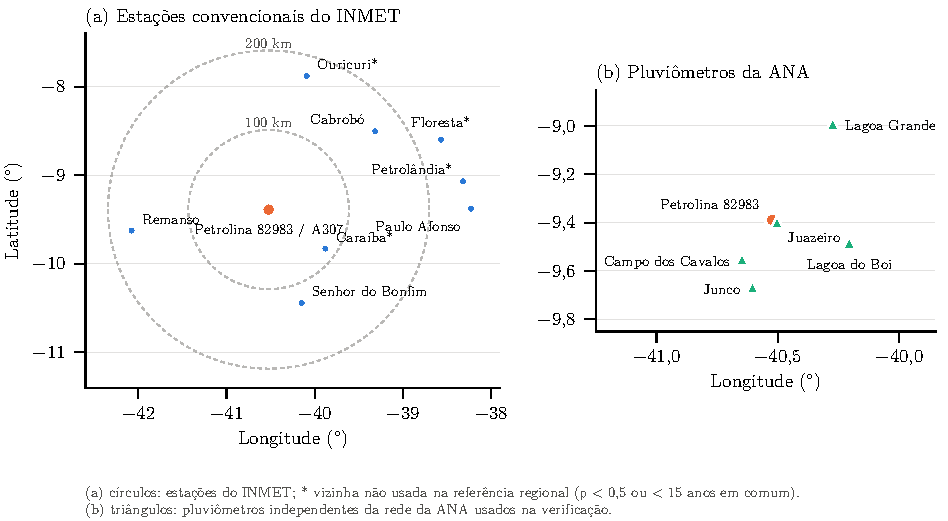
\includegraphics[width=\textwidth]{figuras/fig01_area.pdf}
  \caption{(a) Estação \Est{} (Petrolina; a automática A307 fica no mesmo sítio) e estações
  convencionais vizinhas do INMET, com anéis de 100 e 200~km. (b) Pluviômetros independentes da
  rede da ANA usados na verificação da tendência da chuva (\cref{tab:ana}).}
  \label{fig:area}
\end{figure}

% ============================================================================= dados
\section{Dados}\label{sec:dados}

\subsection{Fontes}
A série principal é a diária da estação convencional \Est{} do INMET, obtida no Banco de
Dados Meteorológicos (BDMEP) para 1961--2025: chuva, temperaturas máxima, mínima e média
compensada, umidade relativa, vento, insolação e evaporação. A estação automática A307, no
mesmo sítio, tem dados horários de 2003 a 2024 e é usada como série de validação. As
estações convencionais vizinhas (\cref{fig:area}) servem de referência regional. Como
verificação independente, usamos também a chuva diária de pluviômetros da rede hidrometeorológica
da Agência Nacional de Águas (ANA), operados por outras instituições e com outros instrumentos,
obtida no serviço Hidroweb. Os índices mensais ONI, TNA e TSA vêm do NOAA Physical Sciences
Laboratory.

\subsection{Critérios de completude}
Um ano hidrológico (julho--junho) é válido se a \emph{fração climatológica ausente} (FCA)
for no máximo 5\,\%. A FCA é a parte da chuva anual esperada, pela climatologia diária de
cada mês, que cairia nos dias sem registro:
\begin{equation}
  \mathrm{FCA} = \frac{\sum_{d\,\in\,\text{ausentes}} \bar c_{m(d)}}{\sum_{m=1}^{12} \bar c_m\, n_m},
\end{equation}
em que $\bar c_m$ é a chuva diária média do mês $m$ em 1991--2020 e $n_m$ o número de dias
do mês. Assim, uma falha em agosto pesa pouco e uma falha em março pesa muito. Para
temperatura usa-se a regra da OMM para meses (no máximo 10 dias ausentes e 4 consecutivos) e
exigem-se 10 meses válidos por ano \parencite{wmo2017}. Dos \NanosHidro{} anos hidrológicos,
\NanosValidos{} são válidos (\PrimeiroAnoValido{} a \UltimoAnoValido{}). Como sensibilidade,
relaxamos o critério para FCA $\le$ 7,5\,\%, o que acrescenta \AnosFCASete{} (FCA de
\FCAumnoveoitoumoitodois{}, \FCAdoiszerodoisumdoisdois{} e \FCAdoiszerodoistresdoisquatro{}\,\%,
respectivamente). O último, um ano chuvoso no fim da série, fica fora do critério principal por
pouco.

\subsection{Qualidade e homogeneidade}
A \cref{fig:ausencias} mostra a fração de dias ausentes por ano e variável, e a
\cref{fig:padroes} mostra quais variáveis faltam juntas. Ambas foram calculadas com
MissingPatterns.jl \parencite{bertuzzi_missingpatterns}. Na A307, o padrão de ausência mais comum é
a falta simultânea de todas as variáveis: quando o registrador para, tudo some, de modo que a
ausência depende do tempo e não do valor medido.

\begin{figure}[htbp]
  \centering
  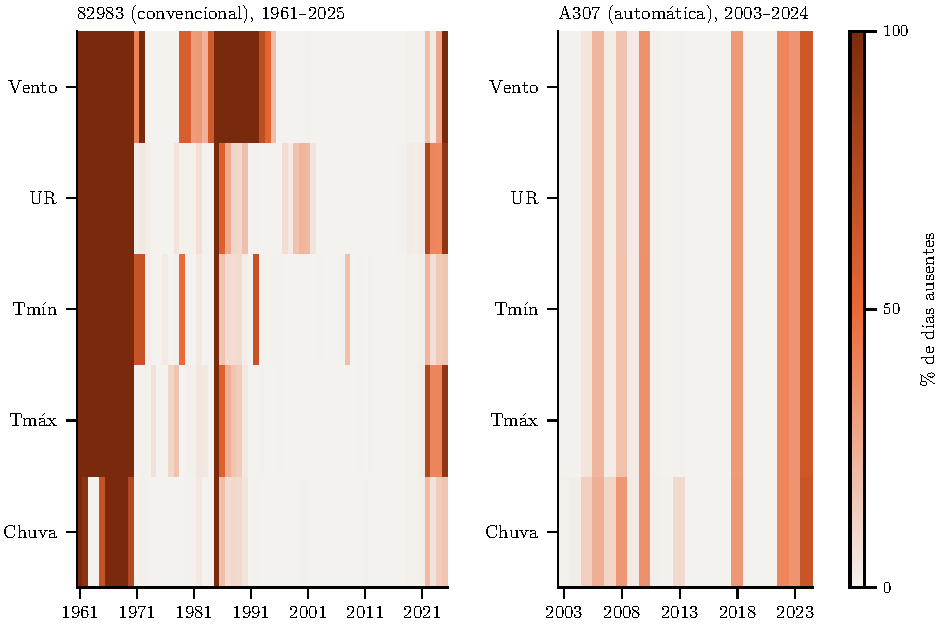
\includegraphics[width=\textwidth]{figuras/fig02_ausencias.pdf}
  \caption{Percentual de dias sem registro por ano e variável. Na \Est{}, temperatura, UR e
  vento anteriores a 1971 foram excluídos por inomogeneidade (\cref{sec:dados}).}
  \label{fig:ausencias}
\end{figure}

\begin{figure}[htbp]
  \centering
  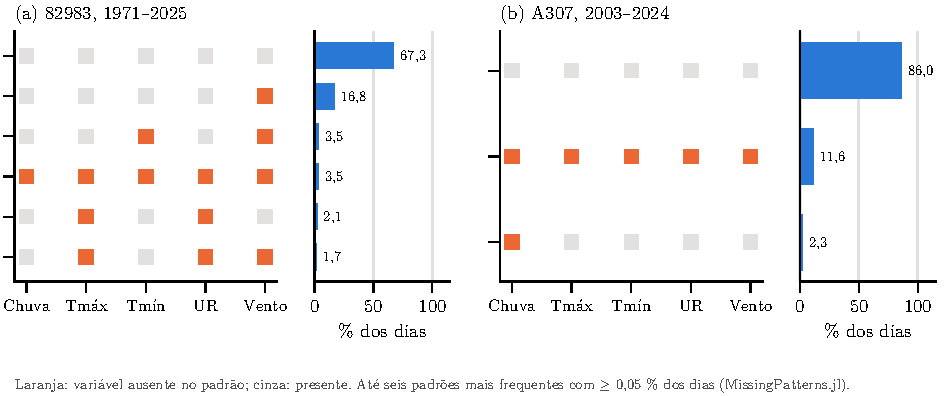
\includegraphics[width=\textwidth]{figuras/fig12_padroes_ausencia.pdf}
  \caption{Padrões de ausência conjunta na escala diária: cada linha é uma combinação de
  variáveis ausentes no mesmo dia, e a barra é a fração de dias com aquele padrão.}
  \label{fig:padroes}
\end{figure}

\paragraph{A307 \texorpdfstring{$\times$}{x} \Est.}
Nos dias em que as duas estações têm registro, a razão anual entre os totais de chuva
(A307/\Est) tem média \RazaoChuvaMedia{} e varia de \RazaoChuvaMin{} a \RazaoChuvaMax{}, sem
quebra detectável (SNHT, $p$\,\PSnhtChuva; Pettitt, $p$\,\PPettittChuva). O valor mínimo,
\RazaoChuvaDozeTreze{}, ocorre justamente em 2012/13: a A307 registrou bem menos chuva que
o pluviômetro convencional naquele ano. Por isso a chuva do artigo vem só da \Est{}: um
único instrumento, sem preenchimento entre fontes. Na temperatura, a diferença média
A307$-$\Est{} é \DifMediaTmax{}~°C na máxima e \DifMediaTmin{}~°C na mínima, com indício de
quebra nas duas (Tmáx: SNHT $p$\,\PSnhtTmax; Tmín: Pettitt $p$\,\PPettittTmin). Esta
comparação não indica qual das duas estações mudou; a \cref{sec:resultados} testa a
sensibilidade das tendências de temperatura a isso.

\paragraph{\Est{} \texorpdfstring{$\times$}{x} vizinhas.}
Como a \Est{} mostrou forte tendência de chuva, testamos se ela é climática ou
instrumental. Construímos uma série de referência ponderada pelas vizinhas, com pesos iguais
ao quadrado da correlação entre primeiras diferenças, e analisamos a razão
$Q_t = Y_t/R_t$ entre a candidata e a referência \parencite{alexandersson1997}. Entraram
\NvizinhasUsadas{} vizinhas; duas delas encerram o registro antes do fim do período, de modo que
a referência dos anos mais recentes depende de menos estações. A referência também tem
tendência negativa, de \SenReferencia{}~mm por década \IC{\SenReferenciaICinf}{\SenReferenciaICsup}
($p$\,\PMKReferencia): a queda é compartilhada pelas vizinhas. A razão $Q$, porém, também
diminui: \SenQ{}\,\% por década \IC{\SenQICinf}{\SenQICsup} ($p$\,\PTendQ), ou seja, a \Est{}
seca mais rápido que a referência. O SNHT e o Pettitt indicam, com significância marginal, uma
quebra após \QuebraQ{} (SNHT $p$\,\PSnhtQ; Pettitt $p$\,\PPettittQ), com $Q$ passando de
\QAntes{} para \QDepois{}. Nenhum dos \Npares{} pares estação a estação, que não sofrem com a
mudança de composição da referência, tem quebra após a correção de Benjamini--Hochberg
\parencite{benjamini1995}. A data coincide com a instalação da estação automática no mesmo sítio,
o que torna plausível, mas não demonstrável com estes dados, uma mudança na rotina ou na
exposição do pluviômetro convencional. A diferença também pode ser um gradiente espacial real.
Por isso a P1 é apresentada também com a inclinação regional, que exclui a parte local da queda.

\paragraph{\Est{} \texorpdfstring{$\times$}{x} pluviômetros da ANA.}
As vizinhas acima são do próprio INMET. Para uma verificação com instrumentos e operadores
diferentes, consideramos \NPostosAnaCandidatos{} pluviômetros da rede da ANA a até cerca de 70~km
de Petrolina, com registro longo. Cada um passou pelo mesmo critério de completude da \Est{}, com
a climatologia do próprio posto, e entraram os \NPostosAna{} com pelo menos \MinComumAna{} anos
hidrológicos válidos em comum com ela. Nos anos comuns, comparamos as tendências e testamos a
razão $Q = Y_{\Est}/Y_{\text{posto}}$ (\cref{tab:ana}). Todos os postos têm tendência negativa, e em
\NAnaNegSig{} deles o intervalo exclui zero, com declives de \SenAnaMin{} a \SenAnaMax{}~mm por
década. O mais informativo é Juazeiro, a \DistJuazeiro{}~km, do outro lado do rio: nos mesmos
\NComumJuazeiro{} anos, ele cai \SenAnaJuazeiro{}~mm por década
\IC{\SenAnaJuazeiroICinf}{\SenAnaJuazeiroICsup}, contra \SenRefJuazeiro{} na \Est{}. A razão entre
os dois não tem tendência ($p$\,\PQAnaJuazeiro) nem muda significativamente entre antes e
depois de 2003/04 ($Q$ de \QAntesAnaJuazeiro{} para \QDepoisAnaJuazeiro{}; $p$\,\PAntesDepoisAnaJuazeiro);
se algo, a \Est{} passa a registrar relativamente mais, o contrário do que uma perda instrumental
produziria. O SNHT
localiza esse aumento em \QuebraAnaJuazeiro{}, o que, se algo, atenua a tendência da \Est{}. Frente a Junco e a Lagoa
Grande, a razão cai (\NAnaQSig{} dos \NPostosAna{} testes com $p<0{,}05$), e frente a Junco também
há diferença antes e depois de 2003/04. Mas a razão com Junco tem sua quebra
principal em \QuebraAnaJunco{}, duas décadas antes da estação automática, Junco tem a menor
tendência do grupo, e os outros três postos não confirmam o excesso local. Em conjunto, os pluviômetros independentes confirmam que a queda da chuva é real e
regional, e não dão apoio consistente a uma mudança instrumental na \Est{} em 2003/04.

\begin{table}[htbp]
  \centering
  \caption{Pluviômetros independentes da rede da ANA: tendência da chuva anual (Sen, mm por
  década, IC de 95\,\%) nos anos hidrológicos válidos em comum com a \Est{}, tendência da \Est{}
  nos mesmos anos e teste de tendência (Mann--Kendall) na razão $Q$ = \Est{}/posto.}
  \label{tab:ana}
  \small
  \begin{tabular}{@{}lrrrrr@{}}
    \toprule
    Posto (operador ANA) & km & $n$ & Sen posto \IC{inf}{sup} & Sen \Est{} & $p$ ($Q$) \\
    \midrule
    Juazeiro & \DistJuazeiro & \NComumJuazeiro & \SenAnaJuazeiro{} \IC{\SenAnaJuazeiroICinf}{\SenAnaJuazeiroICsup} & \SenRefJuazeiro & \PQAnaJuazeiroVal \\
    Campo dos Cavalos & \DistCavalos & \NComumCavalos & \SenAnaCavalos{} \IC{\SenAnaCavalosICinf}{\SenAnaCavalosICsup} & \SenRefCavalos & \PQAnaCavalosVal \\
    Junco & \DistJunco & \NComumJunco & \SenAnaJunco{} \IC{\SenAnaJuncoICinf}{\SenAnaJuncoICsup} & \SenRefJunco & \PQAnaJuncoVal \\
    Lagoa do Boi & \DistLagoaBoi & \NComumLagoaBoi & \SenAnaLagoaBoi{} \IC{\SenAnaLagoaBoiICinf}{\SenAnaLagoaBoiICsup} & \SenRefLagoaBoi & \PQAnaLagoaBoiVal \\
    Lagoa Grande & \DistLagoaGrande & \NComumLagoaGrande & \SenAnaLagoaGrande{} \IC{\SenAnaLagoaGrandeICinf}{\SenAnaLagoaGrandeICsup} & \SenRefLagoaGrande & \PQAnaLagoaGrandeVal \\
    \bottomrule
  \end{tabular}
\end{table}

\paragraph{Temperatura antes de 1971.}
Antes da lacuna de 1966--1970, a Tmáx da \Est{} difere em média \DifIniTmaxCabrobo{}~°C da de
Cabrobó, contra \DifPosTmaxCabrobo{}~°C a partir de 1971 (Remanso: \DifIniTmaxRemanso{} e
\DifPosTmaxRemanso{}~°C). Na Tmín as diferenças iniciais são menores (\DifIniTminCabrobo{} e
\DifIniTminRemanso{}~°C). Como o segmento é curto e isolado por cinco anos sem dados, e a Tmáx
mostra claramente outro padrão de medição, adotamos a opção conservadora de usar temperatura,
UR e vento só a partir de 1971. A chuva desse período é compatível com as vizinhas e foi mantida.

% ============================================================================= métodos
\section{Métodos}\label{sec:metodos}

\subsection{Índices de seca}
\paragraph{SPI.} Para cada escala $k \in \{3, 6, 12\}$ meses, $X_t = \sum_{j=0}^{k-1} P_{t-j}$.
Para cada mês do calendário ajusta-se uma Gamma por máxima verossimilhança aos $X_t>0$ de
1991--2020, com massa $q$ em zero \parencite{mckee1993,guttman1999}:
\begin{equation}
  H(x) = q + (1-q)\,G(x;\alpha,\beta), \qquad \mathrm{SPI}_t = \Phi^{-1}\!\big(H(X_t)\big).
\end{equation}

\paragraph{SPEI.} Sobre o balanço $D_t = P_t - \mathrm{ETo}_t$ \parencite{vicenteserrano2010}.
A radiação medida da A307 foi excluída (mudanças de escala e lacunas), e a \Est{} não
mede radiação. Por isso a evapotranspiração de referência vem de Hargreaves--Samani, que
depende só de Tmáx, Tmín e da radiação extraterrestre $R_a$, função da latitude e do dia
\parencite{hargreaves1985,allen1998}:
\begin{equation}
  \mathrm{ETo} = 0{,}0023 \cdot 0{,}408\,R_a\,(\bar T + 17{,}8)\sqrt{T_{\max} - T_{\min}}.
\end{equation}
Para $D_t$ ajustamos a log-logística de três parâmetros por momentos ponderados por
probabilidade \parencite{vicenteserrano2010} e, como sensibilidade, a GEV por L-momentos
\parencite{hosking1990,stagge2015}. Quando a amostra tem assimetria negativa, a
log-logística é ajustada a $-D_t$.

\paragraph{Teoria de corridas.} Um evento é uma sequência de meses com índice abaixo de
$z_0=-1$, com duração $D$, severidade $S=-\sum z_t$ e intensidade $S/D$
\parencite{yevjevich1967}.

\subsection{Período de retorno}
Seja $x_0$ o total do evento de referência. A probabilidade de um ano igual ou mais seco é
$p = F(x_0)$ e o período de retorno é $T=1/p$. Supondo anos independentes,
\begin{equation}
  P(\text{ao menos um evento em } n \text{ anos}) = 1 - (1-p)^n. \label{eq:pn}
\end{equation}
Comparamos Gamma, Weibull, log-normal e normal por AIC, pesos de Akaike
\parencite{burnham2002} e Anderson--Darling com $p$ por bootstrap paramétrico
\parencite{anderson1954}. Como nenhuma candidata domina, o resultado estacionário principal é a
média de $p$ ponderada pelos pesos de Akaike, com IC por bootstrap não paramétrico dos anos (as
quatro distribuições e os pesos são reajustados a cada réplica). A Gamma, que é a base do SPI e
admite uma parametrização simples para os modelos bayesiano e não estacionário, é usada para os
intervalos por verossimilhança perfilada, reparametrizando por $(k, p)$ com
$\theta = x_0/Q_{\Gamma(k,1)}(p)$ \parencite{coles2001}, por bootstrap paramétrico e por
posterior bayesiana. No modelo bayesiano, $\log k \sim \mathcal N(\log 4, 1)$ e
$\log\mu \sim \mathcal N(\log 500, 1)$, prioris fracamente informativas que cobrem coeficientes
de variação de cerca de 0,2 a 1,3 e médias de cerca de 70 a 3\,500~mm. A sensibilidade foi
testada dobrando os desvios-padrão. A adequação foi checada pelo $\hat R$ \parencite{gelman1992},
pelo tamanho efetivo de amostra e por uma checagem preditiva posterior do mínimo amostral.

Uma ressalva de interpretação: o evento de referência foi escolhido por ser um dos mais extremos
já observados, e ele próprio está na amostra de ajuste. O período de retorno de um evento
selecionado dessa forma deve ser lido como a frequência de anos \emph{ao menos tão secos quanto
o limiar}, e não como uma estimativa não viesada da raridade daquele ano específico.

\paragraph{Não estacionariedade.} O parâmetro de posição de cada candidata passa a variar no
tempo:
\begin{equation}
  \log \lambda_t = a + b\,\tau_t, \qquad \log s_t = s_0 + c\,\tau_t,
\end{equation}
com $\tau_t$ o tempo em décadas centrado, $\lambda_t$ a média (normal e Gamma), a escala
(Weibull) ou a mediana (log-normal), e $s_t$ o parâmetro de forma (o desvio-padrão na normal e
na log-normal). Assim, as quatro candidatas têm a mesma tendência multiplicativa, $e^{b}-1$ por
década. Com $c = 0$ (forma fixa), elas diferem na forma como a variabilidade acompanha a média:
a normal mantém o desvio-padrão constante; a Gamma, a Weibull e a log-normal mantêm o coeficiente
de variação. Com $c$ livre (forma variável), essa relação é estimada a partir dos dados, e a
hipótese de forma fixa é testada por razão de verossimilhança em cada família. Como no caso
estacionário, o resultado principal é a média de $p$ ponderada pelos pesos de Akaike das oito
candidatas não estacionárias (quatro famílias, com forma fixa e variável), com IC por bootstrap
não paramétrico dos anos, em que as oito candidatas e os pesos são reajustados a cada réplica. A Gamma não estacionária,
$Y_t \sim \mathrm{Gamma}(k,\ \mu_t/k)$, também é ajustada de forma bayesiana, com
$b \sim \mathcal N(0,\,0{,}2)$, que admite variações de até cerca de 40\,\% por década, e serve
como sensibilidade. Ela também define os estados sem tendência da persistência e das
teleconexões. O valor principal é avaliado no último ano hidrológico válido; valores para 2025
extrapolam a tendência para além dos dados e são apresentados como cenário. Como sensibilidades,
$b$ é fixado na inclinação estimada para a série de referência regional (de novo como média entre
as candidatas), e a Gamma é reajustada com o critério FCA $\le$ 7,5\,\%. Quando $p$ varia ano a
ano, a \cref{eq:pn} vira $1-\prod_{j=1}^{n}(1-p_{t_0+j})$.

\subsection{Persistência}
Classificamos cada ano hidrológico como seco (tercil inferior) ou não seco e estimamos uma
cadeia de Markov de primeira ordem só com pares de anos consecutivos válidos. Com priori
de Jeffreys, a posterior de cada linha da matriz de transição é Dirichlet$(\tfrac12 + n_{i1},
\tfrac12 + n_{i2})$. Como uma tendência agrupa anos secos mesmo sem persistência, repetimos
a análise com estados definidos pela transformação integral de probabilidade sob o modelo não
estacionário, $u_t = F_t(y_t)$, com seco $\Leftrightarrow u_t \le 1/3$.

\subsection{Teleconexões}
Calculamos a correlação da chuva anual com o ONI e com o gradiente meridional do Atlântico
(TNA$-$TSA), ambos médios de novembro a abril, com IC pela transformação $z$ de Fisher. Como a
chuva tem tendência, repetimos a correlação com a chuva sem tendência (a transformação integral
sob o modelo não estacionário, levada à escala normal), para não confundir tendência com
teleconexão. Estimamos também $P(\text{ano seco} \mid \text{fase do ENSO})$, com fases definidas
por ONI $\ge 0{,}5$ (El Niño), $\le -0{,}5$ (La Niña) e as demais (neutro), por posterior Beta
com priori de Jeffreys.

\subsection{Tendências e mudanças}
Usamos o teste de Mann--Kendall \parencite{mann1945,kendall1975} com pré-branqueamento livre
de tendência \parencite[TFPW;][]{yue2002} como teste principal, a correção de variância de
\textcite{hamed1998} como verificação, o declive de \textcite{sen1968} com IC de 95\,\% e o
teste de \textcite{pettitt1979}. A correção de \textcite{benjamini1995} é aplicada à família de
testes de cada pergunta. Como as séries têm lacunas, o pré-branqueamento usa só pares de anos
realmente consecutivos, em vez de tratar a série compactada como contígua. Para interpretar
resultados não significativos, estimamos por
simulação AR(1) a \emph{tendência mínima detectável} (poder de 80\,\% a 5\,\%). Os índices de
extremos seguem o ETCCDI \parencite{zhang2011}, com percentis por dia do calendário em janelas
de 5 dias no período 1991--2020. Não aplicamos a correção por bootstrap de \textcite{zhang2005}
para os anos dentro do período-base, o que pode introduzir pequenas descontinuidades em TX90p e
TN10p nas bordas desse período. A sazonalidade é descrita pelo índice de \textcite{walsh1981},
pelo centroide e pela concentração circular da chuva diária e pelas datas de início e fim da
estação chuvosa de \textcite{liebmann2007}. Anos em que a anomalia acumulada não atinge um máximo
dentro do ano hidrológico são classificados como \emph{sem estação definida}, e a tendência na
frequência desses anos é testada por regressão logística no tempo. A regressão quantílica
\parencite{koenker1978} da temperatura diária no tempo, com dois harmônicos sazonais, tem IC por
bootstrap em blocos anuais \parencite{kunsch1989}. A decomposição STL \parencite{cleveland1990}
das séries mensais é usada como descrição complementar da tendência.

Toda a análise foi feita em Julia \parencite{bezanson2017}. As figuras usam CairoMakie
\parencite{danisch2021}, e os modelos bayesianos usam Turing \parencite{ge2018} com o amostrador
NUTS \parencite{hoffman2014}. Os métodos sem implementação confiável disponível (SPI, SPEI,
Hargreaves, MK modificado, SNHT, corridas) foram implementados à mão e testados contra valores
publicados \parencite{allen1998} ou contra propriedades conhecidas.

% ============================================================================= resultados
\section{Resultados}\label{sec:resultados}

\subsection{Evento de referência}
A \cref{fig:chuva} mostra a chuva por ano hidrológico. Os anos mais secos válidos são
\RankAnoum{} (\RankChuvaum{}~mm), \RankAnodois{} (\RankChuvadois{}~mm), \RankAnotres{}
(\RankChuvatres{}~mm), \RankAnoquatro{} (\RankChuvaquatro{}~mm) e \RankAnocinco{}
(\RankChuvacinco{}~mm). Os três primeiros caem na sequência seca de 2011/12 a 2016/17. Pelo
total anual, \textbf{2012/13 não é o ano mais seco}: é o \RankDozeTreze{}º, atrás de
\AnoMinimo{}, e está empatado, para todos os fins práticos, com \RankAnotres{}
(\RankChuvadois{} contra \RankChuvatres{}~mm). Pelo SPI-12
de junho, 2016/17 também é o mais extremo (SPI $=\SPIDezesseisDezessete$, contra
$\SPIDozeTreze$ em 2012/13; SPEI-12: $\SPEIDezesseisDezessete$ e $\SPEIDozeTreze$). Definimos
portanto três eventos de referência: \emph{E1}, um ano com chuva $\le$ \ChuvaDozeTreze{}~mm (o
total de 2012/13); \emph{E1$'$}, um ano $\le$ \ChuvaMinima{}~mm (o mínimo do registro); e
\emph{E3}, o evento plurianual de seca no SPI-12 que inclui 2012/13.

\begin{figure}[htbp]
  \centering
  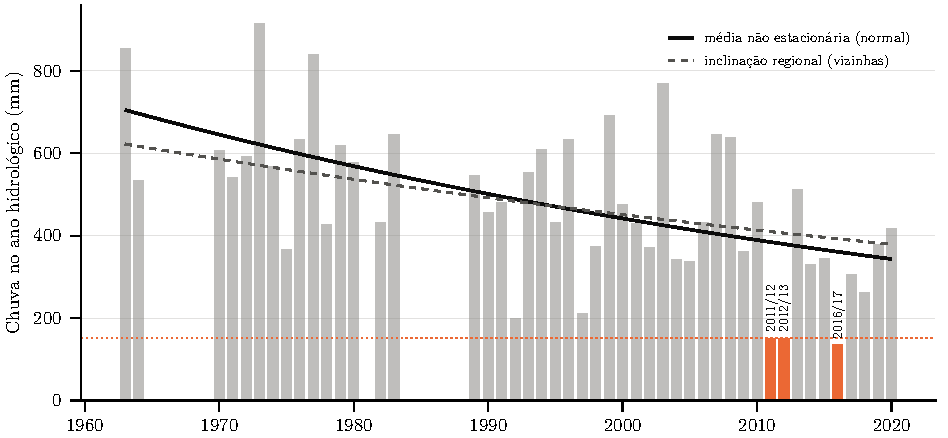
\includegraphics[width=\textwidth]{figuras/fig04_chuva_anual.pdf}
  \caption{Chuva por ano hidrológico na \Est{} (anos válidos). Em laranja, os anos com chuva
  $\le$ 2012/13. Linhas: média da normal não estacionária, a candidata de menor AIC (contínua),
  e média com a inclinação regional (tracejada). As demais candidatas têm médias quase iguais.}
  \label{fig:chuva}
\end{figure}

O SPI-12 tem \NeventosSPI{} eventos em \AnosCobertosSPI{} anos cobertos, todos a partir de 1993
(\cref{fig:spi}). Isso tem duas causas. O SPI-12 exige 12 meses seguidos com dados, e as
lacunas de 1966--1970 e 1985--1991 deixam poucos anos cobertos antes de 1992. E, como a
referência é 1991--2020, mais seca, os anos cobertos das décadas de 1960 a 1980 aparecem
relativamente úmidos: nenhum deles chega a SPI-12 $<-1$. A concentração recente dos eventos
reflete, portanto, tanto a cobertura quanto a tendência, e não deve ser lida como evidência
independente desta. O evento E3 vai de \EvRefInicio{} a \EvRefFim{} (\EvRefDuracao{} meses), com
severidade \EvRefSeveridade{}, intensidade \EvRefIntensidade{} e pico \EvRefPico{}. É o mais
severo do registro. O SPEI-12 identifica os mesmos episódios.

\begin{figure}[htbp]
  \centering
  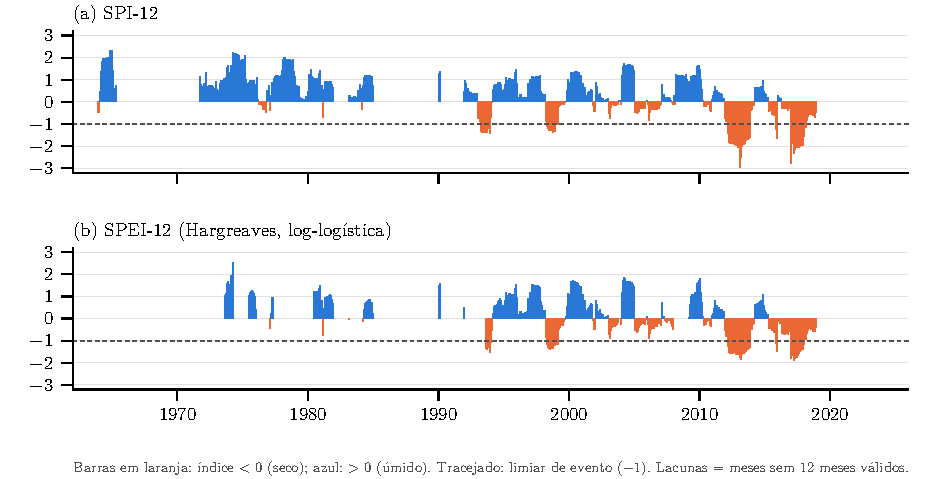
\includegraphics[width=\textwidth]{figuras/fig05_spi_spei.pdf}
  \caption{SPI-12 e SPEI-12 mensais da \Est{} (período de referência 1991--2020).}
  \label{fig:spi}
\end{figure}

\subsection{Período de retorno (P1)}
Com \NanosValidos{} anos, as quatro distribuições candidatas diferem pouco. A de menor AIC é a
\MelhorAIC{}; a Gamma tem peso de Akaike \GammaPesoAkaike{} e $p_{AD}=\GammaPAD$, ou seja, é
aceitável, mas não a melhor. Sob estacionariedade, o período de retorno de E1 vai de \TNormal{}
anos (normal) a \TWeibull{} (Weibull), \TGamma{} (Gamma) e \TLogNormal{} (log-normal); a
log-normal, porém, é rejeitada pelo Anderson--Darling, e entre as candidatas não rejeitadas o
máximo é \TModelosMaxAceitos{} anos. A média ponderada por AIC é de \TMediaAkaikeB{} anos
\IC{\TMediaAkaikeBICinf}{\TMediaAkaikeBICsup} (\cref{tab:retorno}). Empiricamente,
\NanosAteDozeTreze{} dos \NanosValidos{} anos tiveram chuva $\le$ E1
($T \approx \TEmpiricoDozeTreze$ anos pela posição de Weibull), o que indica que a cauda seca da
Gamma é mais fina que a dos dados.

A tendência da chuva anual é forte: \SenChuva{}~mm/década \IC{\SenChuvaICinf}{\SenChuvaICsup}
(MK $p$\,\PMKChuva; TFPW $p$\,\PTFPWChuva). Na Gamma, o modelo não estacionário é claramente
preferido ao estacionário ($\Delta\mathrm{AIC} = \NSTempoDAIC$; razão de verossimilhança
$p$\,\NSTempoP), com variação da média de \NSTempoEfeito{}\,\% por década (bayesiano:
\BayesNSEfeito{}\,\% \IC{\BayesNSEfeitoICinf}{\BayesNSEfeitoICsup}; $P(b<0\mid y) =
\ProbBNegativo$). Mas a hipótese de coeficiente de variação constante, embutida na Gamma, é
rejeitada pelos dados. Deixando a forma variar no tempo, a razão de verossimilhança rejeita a
forma fixa na Gamma ($p$\,\PFormaVarGamma) e na log-normal ($p$\,\PFormaVarLogNormal), é marginal
na Weibull ($p$\,\PFormaVarWeibull) e é desnecessária na normal ($p$\,\PFormaVarNormal), cujo
desvio-padrão fica praticamente constante (\EfeitoFormaNormal{}\,\% por década). Na Gamma, o
parâmetro de forma cai \EfeitoFormaGamma{}\,\% por década, isto é, o coeficiente de variação
cresce. Em outras palavras, a chuva anual diminuiu sem que a amplitude da oscilação interanual em
milímetros diminuísse, o que torna os anos muito secos relativamente mais frequentes.

Essa hipótese pesa muito na cauda. No último ano hidrológico válido (\UltimoAnoNS), com forma
fixa, o período de retorno de E1 vai de \TNSNormal{} anos (normal) a \TNSWeibull{} (Weibull) e
\TNSGamma{} (Gamma). Com forma variável, as quatro famílias convergem: \TNSNormalVar{} (normal),
\TNSWeibullVar{} (Weibull), \TNSGammaVar{} (Gamma) e \TNSLogNormalVar{} anos (log-normal). A
candidata de menor AIC é a \MelhorAICNS{} com forma \MelhorAICNSForma{} (peso \PesoNSNormal{}), e as
versões com forma variável somam peso \PesoNSVarTotal{}. O resultado principal, a média ponderada
pelos pesos de Akaike das oito candidatas, é de \TNSMediaUlt{} anos
\IC{\TNSMediaUltICinf}{\TNSMediaUltICsup}; só com as de forma fixa, \TNSMediaFixaUlt{} anos. Como esse
valor é avaliado no fim de uma década seca, repetimos o ajuste com o critério FCA $\le$ 7,5\,\%,
que inclui os anos chuvosos \AnosFCASete{}: a média de Akaike dá \TNSMediaFCASeteUlt{} anos
\IC{\TNSMediaFCASeteUltICinf}{\TNSMediaFCASeteUltICsup} em \UltimoAnoFCASete{} e
\TNSMediaFCASeteUltStd{} em \UltimoAnoNS{}, de modo que o resultado principal não depende da
exclusão desses anos. Com a inclinação regional, mais lenta
(\NSRegionalEfeito{}\,\% por década), a média entre as candidatas dá \TRegionalMedia{} anos
\IC{\TRegionalMediaICinf}{\TRegionalMediaICsup} em 2025. Comparado no mesmo esquema, o período de
retorno passa de \TMediaAkaikeB{} anos sob estacionariedade para \TNSMediaUlt{} com a média
recente. Dentro da Gamma, a passagem é de \TGamma{} para \TTempoUlt{} anos (máxima
verossimilhança), ou \TBayesNSUlt{} \IC{\TBayesNSUltICinf}{\TBayesNSUltICsup} na versão bayesiana.

\paragraph{Sensibilidade da tendência da chuva.} Como a série válida termina numa década seca e
sem os anos chuvosos que a sucederam, testamos a tendência em subamostras (\cref{tab:senschuva}).
A magnitude é estável: de \SenChuvaAteDezOnze{} a \SenChuvaDesdeSetentaUm{}~mm por década em todas
as versões. Ela não vem só da seca de 2011/12 a 2016/17, pois sem esses anos a queda continua
significativa, embora mais fraca ($p$\,\PTFPWChuvaSemSeca). Também resiste ao critério de
completude mais frouxo, que inclui os anos chuvosos \AnosFCASete{}, e não depende do início da
série. A significância, porém, depende da década de 2010: com os dados só até 2010/11, o
intervalo inclui zero e o teste não rejeita a ausência de tendência ($p$\,\PTFPWChuvaAteDezOnze).
A queda já estava em curso antes da última década, mas só se torna detectável com ela. Uma
tendência linear descreve a série melhor que um degrau único no melhor ponto de corte
(\AnoDegrauChuva; AIC \AICChuvaLinear{} contra \AICChuvaDegrau{}), o que favorece a leitura de
mudança gradual em vez de um único salto. Isso não exclui uma contribuição instrumental parcial,
como a discutida na \cref{sec:dados}.

\begin{table}[htbp]
  \centering
  \caption{Sensibilidade da tendência da chuva anual (declive de Sen, mm por década, IC de 95\,\%;
  $p$ do Mann--Kendall com pré-branqueamento).}
  \label{tab:senschuva}
  \small
  \begin{tabular}{@{}lrrr@{}}
    \toprule
    Amostra & $n$ & Sen \IC{inf}{sup} & $p$ \\
    \midrule
    Todos os anos válidos & \NanosValidos & \SenChuva{} \IC{\SenChuvaICinf}{\SenChuvaICsup} & \PTFPWChuvaVal \\
    Sem 2011/12--2016/17 & \NChuvaSemSeca & \SenChuvaSemSeca{} \IC{\SenChuvaSemSecaICinf}{\SenChuvaSemSecaICsup} & \PTFPWChuvaSemSecaVal \\
    Até 2010/11 & \NChuvaAteDezOnze & \SenChuvaAteDezOnze{} \IC{\SenChuvaAteDezOnzeICinf}{\SenChuvaAteDezOnzeICsup} & \PTFPWChuvaAteDezOnzeVal \\
    A partir de 1971/72 & \NChuvaDesdeSetentaUm & \SenChuvaDesdeSetentaUm{} \IC{\SenChuvaDesdeSetentaUmICinf}{\SenChuvaDesdeSetentaUmICsup} & \PTFPWChuvaDesdeSetentaUmVal \\
    FCA $\le$ 7,5\,\% & \NChuvaFCASete & \SenChuvaFCASete{} \IC{\SenChuvaFCASeteICinf}{\SenChuvaFCASeteICsup} & \PTFPWChuvaFCASeteVal \\
    \bottomrule
  \end{tabular}
\end{table}

Os modelos bayesianos, todos Gamma, convergiram ($\hat R \le \RhatMaxNS$; tamanho efetivo de
amostra $\ge \ESSMin$). A probabilidade preditiva de um mínimo simulado ser menor que o observado
é \PPCMinEst{} no modelo estacionário e \PPCMinNS{} no não estacionário, mas essa checagem do
mínimo dentro da amostra é um teste fraco: ela não detecta a hipótese de coeficiente de variação
constante, rejeitada acima. Por isso os modelos bayesianos servem como sensibilidade à forma de
quantificar a incerteza, não à escolha da distribuição.

\paragraph{Validação fora da amostra.} Para testar os modelos com dados que eles não viram,
ajustamos todos só com os \NTreino{} anos válidos até \AnoCorteValidacao{} e comparamos o número
esperado de anos secos nos \NTeste{} anos válidos seguintes (\PrimeiroAnoTeste{} a
\UltimoAnoTeste{}) com o observado, extrapolando a tendência dos modelos não estacionários
(\cref{tab:valid}). Usamos dois limiares. O percentil 10 do período de ajuste
(\LimiarPdez{}~mm) não depende do período de teste: houve \ObsPdez{} anos abaixo dele, contra
cerca de \EspPdezEstMedia{} esperados pelos modelos estacionários ($p$\,\PObsPdezEstMedia{} de ver
tantos) e de \EspPdezNSGamma{} a \EspPdezNSMedia{} pelos não estacionários
($p$\,\PObsPdezNSMedia{} na média de Akaike). O limiar E1 tem viés de seleção, porque 2012/13 foi
escolhido justamente por ser um ano extremo do período de teste; mesmo assim, ele discrimina a
cauda dos modelos. Houve \ObsEum{} anos $\le$ E1. A Gamma com coeficiente de variação constante
esperava \EspEumNSGamma{} ($p$\,\PObsEumNSGamma), e a média de Akaike não estacionária,
\EspEumNSMedia{} ($p$\,\PObsEumNSMedia). A validação confirma, portanto, a não estacionariedade
com um limiar não viesado e indica que a Gamma de forma fixa subestima a cauda seca.

\begin{table}[htbp]
  \centering
  \caption{Validação fora da amostra: número esperado de anos com chuva abaixo do limiar nos
  \NTeste{} anos válidos de \PrimeiroAnoTeste{} a \UltimoAnoTeste{}, com os modelos ajustados até
  \AnoCorteValidacao{}, e probabilidade de observar ao menos o número registrado (soma de
  Bernoullis independentes). E1 tem viés de seleção (ver texto).}
  \label{tab:valid}
  \small
  \begin{tabular}{@{}lrrrr@{}}
    \toprule
    & \multicolumn{2}{c}{P10 (\LimiarPdez{}~mm)} & \multicolumn{2}{c}{E1 (\ChuvaDozeTreze{}~mm)} \\
    \cmidrule(lr){2-3}\cmidrule(l){4-5}
    Modelo & esperado & $p$ & esperado & $p$ \\
    \midrule
    Observado & \ObsPdez & & \ObsEum & \\
    Gamma estacionária & \EspPdezEstGamma & \PObsPdezEstGammaVal & \EspEumEstGamma & \PObsEumEstGammaVal \\
    Média de Akaike estacionária & \EspPdezEstMedia & \PObsPdezEstMediaVal & \EspEumEstMedia & \PObsEumEstMediaVal \\
    Gamma não estacionária (CV fixo) & \EspPdezNSGamma & \PObsPdezNSGammaVal & \EspEumNSGamma & \PObsEumNSGammaVal \\
    Normal não estacionária (DP fixo) & \EspPdezNSNormal & \PObsPdezNSNormalVal & \EspEumNSNormal & \PObsEumNSNormalVal \\
    Média de Akaike não estacionária & \EspPdezNSMedia & \PObsPdezNSMediaVal & \EspEumNSMedia & \PObsEumNSMediaVal \\
    \bottomrule
  \end{tabular}
\end{table}

\begin{table}[htbp]
  \centering
  \caption{Período de retorno (anos) de um ano hidrológico com chuva $\le$ 2012/13 (E1).
  Intervalos de 95\,\%. As médias por pesos de Akaike usam as quatro candidatas no caso
  estacionário e oito (quatro famílias, com forma fixa e variável) no não estacionário, reajustadas
  a cada réplica do bootstrap dos anos.}
  \label{tab:retorno}
  \small
  \begin{tabular}{@{}llr@{}}
    \toprule
    Modelo & Método do intervalo & $T$ \\
    \midrule
    \multicolumn{3}{@{}l}{\emph{Estacionário}} \\
    Média por pesos de Akaike & bootstrap dos anos & \TMediaAkaikeB{} \IC{\TMediaAkaikeBICinf}{\TMediaAkaikeBICsup} \\
    Gamma & verossimilhança perfilada & \TDozeTreze{} \IC{\TDozeTrezeICinf}{\TDozeTrezeICsup} \\
    Gamma & bootstrap paramétrico & \TBootDozeTreze{} \IC{\TBootDozeTrezeICinf}{\TBootDozeTrezeICsup} \\
    Gamma & posterior (priori base) & \TBayes{} \IC{\TBayesICinf}{\TBayesICsup} \\
    Gamma & posterior (priori vaga) & \TBayesVaga{} \IC{\TBayesVagaICinf}{\TBayesVagaICsup} \\
    \midrule
    \multicolumn{3}{@{}l}{\emph{Não estacionário, \UltimoAnoNS{}}} \\
    Média por pesos de Akaike & bootstrap dos anos & \TNSMediaUlt{} \IC{\TNSMediaUltICinf}{\TNSMediaUltICsup} \\
    Normal / Weibull / Gamma, forma fixa & máxima verossimilhança & \TNSNormal{} / \TNSWeibull{} / \TNSGamma{} \\
    Normal / Weibull / Gamma, forma variável & máxima verossimilhança & \TNSNormalVar{} / \TNSWeibullVar{} / \TNSGammaVar{} \\
    Gamma & posterior & \TBayesNSUlt{} \IC{\TBayesNSUltICinf}{\TBayesNSUltICsup} \\
    Média por pesos de Akaike, FCA $\le$ 7,5\,\% (\UltimoAnoFCASete) & bootstrap dos anos & \TNSMediaFCASeteUlt{} \IC{\TNSMediaFCASeteUltICinf}{\TNSMediaFCASeteUltICsup} \\
    Gamma, FCA $\le$ 7,5\,\% (\UltimoAnoFCASete) & máxima verossimilhança & \TFCASeteUlt{} \\
    \midrule
    \multicolumn{3}{@{}l}{\emph{Não estacionário, 2025 (cenário)}} \\
    Média por pesos de Akaike, inclinação local & bootstrap dos anos & \TNSMediaDoisMilVinteCinco{} \IC{\TNSMediaDoisMilVinteCincoICinf}{\TNSMediaDoisMilVinteCincoICsup} \\
    Média por pesos de Akaike, inclinação regional & bootstrap dos anos & \TRegionalMedia{} \IC{\TRegionalMediaICinf}{\TRegionalMediaICsup} \\
    Gamma, inclinação local & posterior & \TBayesNS{} \IC{\TBayesNSICinf}{\TBayesNSICsup} \\
    Gamma, inclinação regional & máxima verossimilhança & \TRegionalDoisMilVinteCinco{} \\
    \midrule
    Só \PeriodoCurto{} (\NanosCurto{} anos) & Gamma, perfilada & \TCurto{} \IC{\TCurtoICinf}{\TCurtoICsup} \\
    \bottomrule
  \end{tabular}
\end{table}

A \cref{fig:retorno} mostra o efeito da não estacionariedade: com a média do último ano válido,
a curva de retorno se desloca para baixo, e a média de Akaike fica abaixo da Gamma na cauda seca.
A \cref{fig:posterior} mostra o mesmo deslocamento na posterior da Gamma bayesiana. Para o mínimo do registro (E1$'$), o modelo Gamma estacionário dá $T=\TMinimo{}$
anos \IC{\TMinimoICinf}{\TMinimoICsup}. Ajustando só os \NanosCurto{} anos válidos de
\PeriodoCurto{}, o período de retorno de E1 seria de \TCurto{} anos \IC{\TCurtoICinf}{\TCurtoICsup}.
Esse valor reflete apenas o período recente e mais seco e não pode ser obtido sem a série longa,
que é o que permite separar tendência de variabilidade.

\begin{figure}[htbp]
  \centering
  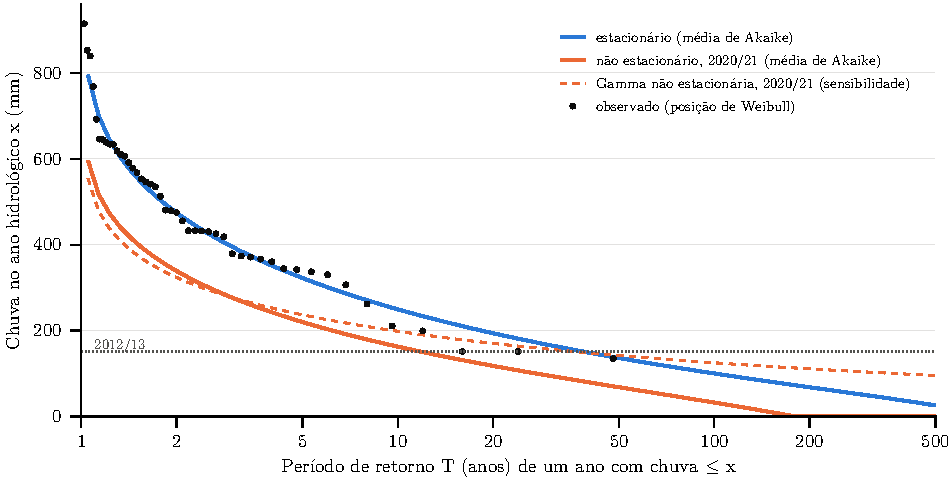
\includegraphics[width=\textwidth]{figuras/fig06_periodo_retorno.pdf}
  \caption{Curva de período de retorno da chuva anual (cauda seca): médias por pesos de Akaike
  estacionária e não estacionária (no último ano válido) e, como sensibilidade, a Gamma não
  estacionária. Pontos: anos observados. A curva não estacionária chega a zero perto de 200 anos
  porque a normal admite valores negativos; só a parte em torno dos limiares do texto é
  interpretável. Os intervalos estão na \cref{tab:retorno}.}
  \label{fig:retorno}
\end{figure}

\begin{figure}[htbp]
  \centering
  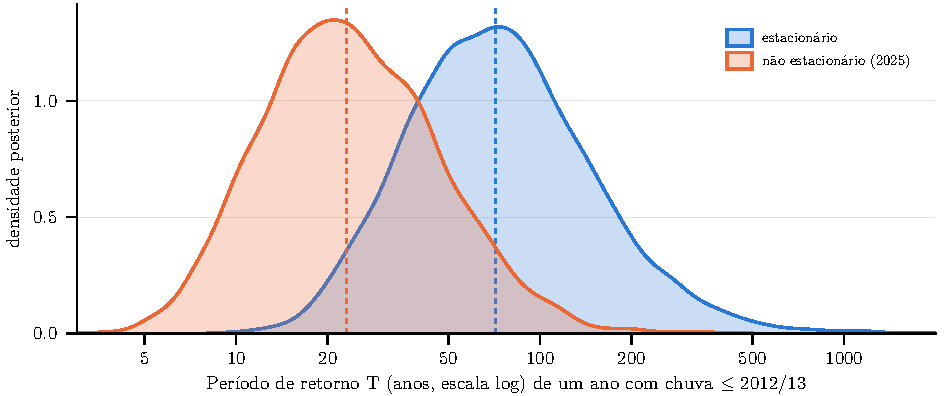
\includegraphics[width=\textwidth]{figuras/fig07_posterior_T.pdf}
  \caption{Posterior do período de retorno de E1 sob os modelos Gamma estacionário e não
  estacionário (cenário de 2025). Tracejado: medianas. A média entre candidatas
  (\cref{tab:retorno}) dá valores menores que a Gamma.}
  \label{fig:posterior}
\end{figure}

A \cref{tab:prob} traduz $T$ em probabilidade de pelo menos um ano igual ou mais seco que
2012/13 nos próximos $n$ anos, sob a hipótese de anos independentes. Sob estacionariedade, a
probabilidade em 30 anos é de \ProbMediaAkaikeNtreszero{}\,\%
\IC{\ProbMediaAkaikeNtreszeroICinf}{\ProbMediaAkaikeNtreszeroICsup}. Mantido o clima do último ano
observado, ela é de \ProbNSMediaUltNtreszero{}\,\%
\IC{\ProbNSMediaUltNtreszeroICinf}{\ProbNSMediaUltNtreszeroICsup}. Esse número supõe o
clima congelado no nível de \UltimoAnoNS{}, ao fim de uma década
excepcionalmente seca, e o intervalo largo mostra o quanto ele é incerto; com só a inclinação regional,
\ProbRegMediaNtreszero{}\,\% \IC{\ProbRegMediaNtreszeroICinf}{\ProbRegMediaNtreszeroICsup}. As
linhas da Gamma bayesiana mostram a sensibilidade à distribuição. O cenário em que a tendência
continua depois de 2025 extrapola uma tendência log-linear para além do período observado e
aparece apenas como limite superior condicional, e não como projeção climática.

\begin{table}[htbp]
  \centering
  \caption{Probabilidade (\%) de ao menos um ano com chuva $\le$ 2012/13 nos próximos $n$ anos.
  Média por pesos de Akaike: IC por bootstrap dos anos. Gamma: posterior bayesiana, com o clima
  mantido no nível do ano indicado ou com a tendência continuada.}
  \label{tab:prob}
  \small
  \begin{tabular}{@{}lcccc@{}}
    \toprule
    Cenário & $n=5$ & $n=10$ & $n=20$ & $n=30$ \\
    \midrule
    \multicolumn{5}{@{}l}{\emph{Média por pesos de Akaike}} \\
    Estacionário & \ProbMediaAkaikeNcinco{} \IC{\ProbMediaAkaikeNcincoICinf}{\ProbMediaAkaikeNcincoICsup}
                 & \ProbMediaAkaikeNumzero{} \IC{\ProbMediaAkaikeNumzeroICinf}{\ProbMediaAkaikeNumzeroICsup}
                 & \ProbMediaAkaikeNdoiszero{} \IC{\ProbMediaAkaikeNdoiszeroICinf}{\ProbMediaAkaikeNdoiszeroICsup}
                 & \ProbMediaAkaikeNtreszero{} \IC{\ProbMediaAkaikeNtreszeroICinf}{\ProbMediaAkaikeNtreszeroICsup} \\
    Clima de \UltimoAnoNS{} mantido & \ProbNSMediaUltNcinco{} \IC{\ProbNSMediaUltNcincoICinf}{\ProbNSMediaUltNcincoICsup}
                 & \ProbNSMediaUltNumzero{} \IC{\ProbNSMediaUltNumzeroICinf}{\ProbNSMediaUltNumzeroICsup}
                 & \ProbNSMediaUltNdoiszero{} \IC{\ProbNSMediaUltNdoiszeroICinf}{\ProbNSMediaUltNdoiszeroICsup}
                 & \ProbNSMediaUltNtreszero{} \IC{\ProbNSMediaUltNtreszeroICinf}{\ProbNSMediaUltNtreszeroICsup} \\
    Inclinação regional, 2025 & \ProbRegMediaNcinco{} \IC{\ProbRegMediaNcincoICinf}{\ProbRegMediaNcincoICsup}
                 & \ProbRegMediaNumzero{} \IC{\ProbRegMediaNumzeroICinf}{\ProbRegMediaNumzeroICsup}
                 & \ProbRegMediaNdoiszero{} \IC{\ProbRegMediaNdoiszeroICinf}{\ProbRegMediaNdoiszeroICsup}
                 & \ProbRegMediaNtreszero{} \IC{\ProbRegMediaNtreszeroICinf}{\ProbRegMediaNtreszeroICsup} \\
    \midrule
    \multicolumn{5}{@{}l}{\emph{Gamma (sensibilidade)}} \\
    Estacionário & \ProbDozeTrezeNcinco{} \IC{\ProbDozeTrezeNcincoICinf}{\ProbDozeTrezeNcincoICsup}
                 & \ProbDozeTrezeNumzero{} \IC{\ProbDozeTrezeNumzeroICinf}{\ProbDozeTrezeNumzeroICsup}
                 & \ProbDozeTrezeNdoiszero{} \IC{\ProbDozeTrezeNdoiszeroICinf}{\ProbDozeTrezeNdoiszeroICsup}
                 & \ProbDozeTrezeNtreszero{} \IC{\ProbDozeTrezeNtreszeroICinf}{\ProbDozeTrezeNtreszeroICsup} \\
    Clima de \UltimoAnoNS{} mantido & \ProbNSUltNcinco{} \IC{\ProbNSUltNcincoICinf}{\ProbNSUltNcincoICsup}
                 & \ProbNSUltNumzero{} \IC{\ProbNSUltNumzeroICinf}{\ProbNSUltNumzeroICsup}
                 & \ProbNSUltNdoiszero{} \IC{\ProbNSUltNdoiszeroICinf}{\ProbNSUltNdoiszeroICsup}
                 & \ProbNSUltNtreszero{} \IC{\ProbNSUltNtreszeroICinf}{\ProbNSUltNtreszeroICsup} \\
    Tendência continua & \ProbNSContNcinco{} \IC{\ProbNSContNcincoICinf}{\ProbNSContNcincoICsup}
                 & \ProbNSContNumzero{} \IC{\ProbNSContNumzeroICinf}{\ProbNSContNumzeroICsup}
                 & \ProbNSContNdoiszero{} \IC{\ProbNSContNdoiszeroICinf}{\ProbNSContNdoiszeroICsup}
                 & \ProbNSContNtreszero{} \IC{\ProbNSContNtreszeroICinf}{\ProbNSContNtreszeroICsup} \\
    \bottomrule
  \end{tabular}
\end{table}

Para o evento plurianual E3, a severidade observada foi a maior entre os \NeventosSPI{} eventos.
Com taxa de \TaxaEventos{} eventos por década e severidade exponencial, o período de retorno de
um evento ao menos tão severo é da ordem de \TSeveridadeRef{} anos (empírico: \TSeveridadeEmp{}).
Com um único evento dessa magnitude, esta estimativa é frágil e serve apenas como ordem de
grandeza.

\subsection{Persistência (P1)}
Com a definição direta (tercil inferior, corte em \CorteSeco{}~mm), $P(\text{seco}\mid
\text{seco}) = \PSS$ \IC{\PSSICinf}{\PSSICsup} e $P(\text{seco}\mid\text{não seco}) = \PNS$
\IC{\PNSICinf}{\PNSICsup}, com probabilidade posterior \ProbPersistencia{} de haver persistência
(\cref{fig:markov}a). Quando os estados são definidos sem a tendência, os valores passam a
\PSSdet{} \IC{\PSSdetICinf}{\PSSdetICsup} e \PNSdet{} \IC{\PNSdetICinf}{\PNSdetICsup}, e a
probabilidade de persistência cai para \ProbPersistenciaDet{} (\cref{fig:markov}b). O resultado
não depende da Gamma usada para remover a tendência: com a normal não estacionária, a candidata de
menor AIC, os valores são \PSSdetNormal{} \IC{\PSSdetNormalICinf}{\PSSdetNormalICsup} e
\PNSdetNormal{} \IC{\PNSdetNormalICinf}{\PNSdetNormalICsup}, com probabilidade de persistência
\ProbPersistenciaDetNormal{}. Os anos
secos de 2011/12 a 2016/17 são, portanto, compatíveis com a queda da média sem memória adicional
de um ano para o outro. Esse resultado tem pouco poder. Há poucas transições observadas, e a
tendência usada para definir os estados foi ajustada aos mesmos dados, de modo que ela absorve
parte de qualquer agrupamento de anos secos. Com estes dados, tendência e persistência
praticamente não se separam: o que se pode afirmar é que não há evidência de persistência além
da tendência, e não que ela esteja ausente.

\begin{figure}[htbp]
  \centering
  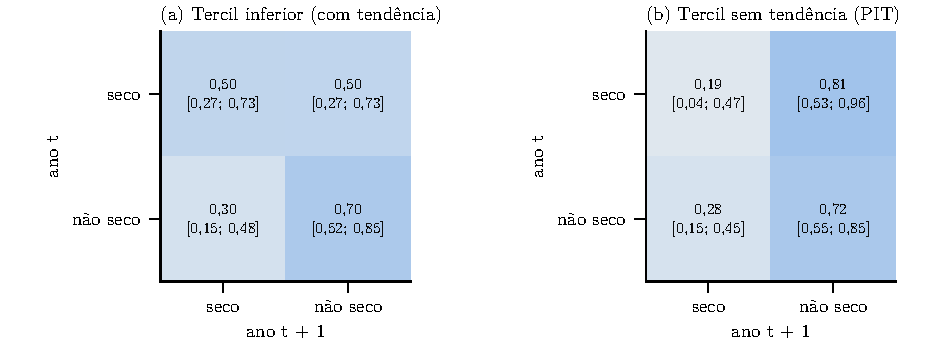
\includegraphics[width=\textwidth]{figuras/fig08_markov.pdf}
  \caption{Matriz de transição (mediana posterior e intervalo de 95\,\%), com estados definidos
  (a) pelo tercil inferior bruto e (b) pelo tercil sob o modelo não estacionário.}
  \label{fig:markov}
\end{figure}

\subsection{Teleconexões (P1)}
A chuva anual tem correlação negativa, mas não significativa, com o ONI de novembro a abril
($r = \ROniBruta$ \IC{\ROniBrutaICinf}{\ROniBrutaICsup}; $q$\,\QOniBruta) e com o gradiente
TNA$-$TSA ($r = \RGradBruta$ \IC{\RGradBrutaICinf}{\RGradBrutaICsup}; $q$\,\QGradBruta). As
correlações têm o sinal esperado e praticamente não mudam sem a tendência ($r = \ROniDet$ e
$\RGradDet$; com a tendência removida pela normal, $\ROniDetNormal$ e $\RGradDetNormal$), ou seja,
o sinal do ENSO não vem da tendência. As probabilidades condicionais são
instáveis. Na série bruta, a probabilidade de ano seco parece maior com El Niño (\PSecoNino{}
\IC{\PSecoNinoICinf}{\PSecoNinoICsup}, \NSecosNino{} de \NFaseNino{} anos) do que em anos neutros
(\PSecoNeutro{} \IC{\PSecoNeutroICinf}{\PSecoNeutroICsup}); sem a tendência, passa a
\PSecoNinoDet{} (\NSecosNinoDet{} de \NFaseNinoDet{} anos), contra \PSecoNeutroDet{} nos neutros.
Com \NFaseNino{} a \NFaseNeutro{} anos por fase, mudar a classificação de poucos anos altera muito essas
proporções, e os intervalos se sobrepõem amplamente nos dois casos.

\subsection{Mudanças no regime (P2)}
\paragraph{Climatologia e sazonalidade.} A \cref{fig:clima} resume o ciclo anual. Na mediana,
a estação chuvosa começa em \InicioMediano{} e termina em \FimMediano{}, com \DuracaoMediana{}
dias. O índice de sazonalidade médio é \SIMedio{} e a concentração circular média é
\ConcMedia{}; nenhum dos dois mostra tendência (TFPW: $p$\,\PTFPWSI{} e $p$\,\PTFPWConc). Em
\NanosSemEstacao{} anos não houve estação chuvosa definida (\AnosSemEstacao). A frequência desses
anos não tem tendência significativa (razão de chances \ORSemEstacao{} por década
\IC{\ORSemEstacaoICinf}{\ORSemEstacaoICsup}; $p$\,\PSemEstacao). Nos demais anos, a evidência
sobre as datas é mista (\cref{fig:estacao}). O início atrasa \SenInicio{} dias por década
\IC{\SenInicioICinf}{\SenInicioICsup} (MK $p$\,\PMKInicio; Hamed--Rao $p$\,\PHRInicio; TFPW
$p$\,\PTFPWInicio), e a duração varia \SenDuracao{} dias por década
\IC{\SenDuracaoICinf}{\SenDuracaoICsup} (MK $p$\,\PMKDuracao; Hamed--Rao $p$\,\PHRDuracao; TFPW
$p$\,\PTFPWDuracao). Os dois IC de Sen excluem zero, e só o teste com pré-branqueamento não é
significativo. Como a tendência mínima detectável do início (\MDTInicio{} dias por década) é
maior que o efeito estimado, a não significância no TFPW reflete falta de poder, e não ausência
de mudança: há indício de uma estação chuvosa que começa mais tarde e é mais curta. Essas
tendências descrevem só os anos com estação definida. Os anos sem estação (\AnosSemEstacao) são
secos e se concentram no período recente; ficando de fora, tendem a fazer a mudança nas datas
parecer menor do que é.

\begin{figure}[htbp]
  \centering
  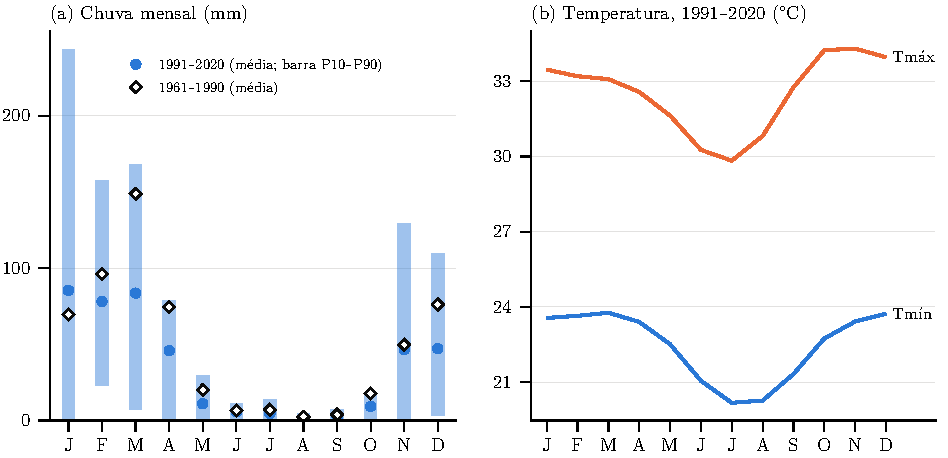
\includegraphics[width=\textwidth]{figuras/fig03_climatologia.pdf}
  \caption{Climatologia mensal da \Est{}. (a) Chuva média de 1991--2020 com faixa P10--P90 e
  média de 1961--1990. (b) Temperaturas máxima e mínima médias de 1991--2020.}
  \label{fig:clima}
\end{figure}

\begin{figure}[htbp]
  \centering
  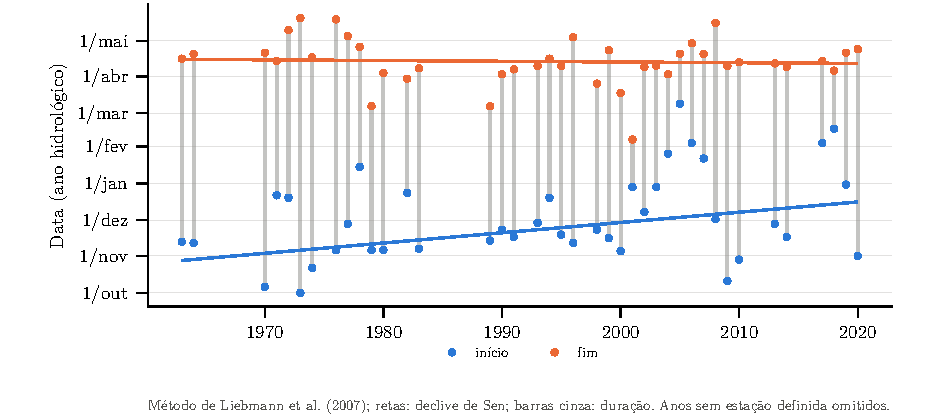
\includegraphics[width=\textwidth]{figuras/fig10_estacao_chuvosa.pdf}
  \caption{Início e fim da estação chuvosa \parencite{liebmann2007} nos anos com estação
  definida.}
  \label{fig:estacao}
\end{figure}

\paragraph{Tendências.} Dos \NtendTotal{} indicadores testados, \NtendSig{} têm $q<0{,}05$
(\cref{tab:tend,fig:tend}), entre eles o vento, que não interpretamos climaticamente (ver
adiante). A temperatura mínima subiu \SenTmin{}~°C por década
\IC{\SenTminICinf}{\SenTminICsup} e a máxima, \SenTmax{} \IC{\SenTmaxICinf}{\SenTmaxICsup}. Como a
comparação com a A307 sugere uma quebra por volta de 2009, repetimos a análise só até 2008: a
Tmín ainda sobe \SenTminAteDoisMilOito{}~°C por década
\IC{\SenTminAteDoisMilOitoICinf}{\SenTminAteDoisMilOitoICsup} e a Tmáx,
\SenTmaxAteDoisMilOito{} \IC{\SenTmaxAteDoisMilOitoICinf}{\SenTmaxAteDoisMilOitoICsup}.

A comparação com as vizinhas depois de 1971 aponta quebras só na Tmáx (\NquebrasTemp{} dos
\NtestesTemp{} testes): frente a Cabrobó, a diferença sobe \SaltoTmaxCabrobo{}~°C a partir de
\QuebraTmaxCabrobo{} ($q$\,\QQuebraTmaxCabrobo), e frente a Remanso, \SaltoTmaxRemanso{}~°C a
partir de \QuebraTmaxRemanso{} ($q$\,\QQuebraTmaxRemanso). A Tmín não tem quebra significativa
frente a nenhuma das duas ($q$\,\QQuebraTminCabrobo{} e $q$\,\QQuebraTminRemanso). O corte em 2008
não elimina a quebra de \QuebraTmaxCabrobo{}, então testamos a Tmáx sob três hipóteses. Se a
\Est{} mudou, subtraindo o salto a partir de \QuebraTmaxCabrobo{}, a tendência é
\SenTmaxAjustada{}~°C por década \IC{\SenTmaxAjustadaICinf}{\SenTmaxAjustadaICsup}
($p$\,\PTFPWTmaxAjustada). Num ajuste agnóstico, com tendência e degrau na mesma data por mínimos
quadrados, ela é \BTmaxDegrau{} \IC{\BTmaxDegrauICinf}{\BTmaxDegrauICsup}, e o degrau estimado é
de só \DegrauTmax{}~°C. A quebra de \QuebraTmaxRemanso{} fica no início da série, e a Tmáx de
1973 também destoa de Cabrobó; começando em 1975, a Tmáx sobe \SenTmaxDesdeSetentaCinco{}
\IC{\SenTmaxDesdeSetentaCincoICinf}{\SenTmaxDesdeSetentaCincoICsup} e a Tmín,
\SenTminDesdeSetentaCinco{} \IC{\SenTminDesdeSetentaCincoICinf}{\SenTminDesdeSetentaCincoICsup}~°C
por década. O aquecimento da Tmáx se mantém em todas as hipóteses, mas sua magnitude é incerta
entre cerca de \SenTmaxAjustada{} e \SenTmaxDesdeSetentaCinco{}~°C por década. A Tmín, sem quebra
frente às vizinhas, é o resultado de temperatura mais firme.

A frequência
de noites frias (TN10p) variou \SenTNumzerop{} pontos percentuais por década e a de dias quentes
(TX90p), \SenTXnovezerop{}. Na chuva, caem os índices de intensidade, Rx1day
(\SenRxumday{}~mm/década), SDII (\SenSDII{}~mm/dia/década) e R95p (\SenRnovecincop{}~mm/década),
mas também a frequência: o número de dias com chuva (R1mm) varia \SenRummm{} dias por década
\IC{\SenRummmICinf}{\SenRummmICsup} ($q$ Hamed--Rao \QHRRummmVal; $q$ TFPW \QTFPWRummmVal).
A amplitude térmica, a UR, o CDD e o CWD não mostram tendência detectável. O vento variou
\SenVento{}~m/s por década. Como quedas de vento em estações convencionais muitas vezes vêm de
mudanças no anemômetro ou no entorno, não interpretamos esse resultado climaticamente. A
decomposição STL das séries mensais (de \STLMesesTmin{} meses, dos quais \STLPreenchTmin{} foram
preenchidos com a climatologia) dá uma variação da componente de tendência de \STLDeltaTmin{}~°C
na Tmín e \STLDeltaTmax{}~°C na Tmáx entre 1971 e 2025, coerente com os declives de Sen.

\begin{table}[htbp]
  \centering
  \caption{Tendências por década (declive de Sen, IC de 95\,\%), $q$ de Benjamini--Hochberg
  sobre o MK-TFPW e tendência mínima detectável (TMD; poder de 80\,\%).}
  \label{tab:tend}
  \small
  \begin{tabular}{@{}llrcr@{}}
    \toprule
    Indicador & Período & Sen \IC{inf}{sup} & $q$ & TMD \\
    \midrule
    Tmáx (°C) & \PeriodoTmax & \SenTmax{} \IC{\SenTmaxICinf}{\SenTmaxICsup} & \QTFPWTmaxVal & \MDTTmax \\
    Tmín (°C) & \PeriodoTmin & \SenTmin{} \IC{\SenTminICinf}{\SenTminICsup} & \QTFPWTminVal & \MDTTmin \\
    Tméd (°C) & \PeriodoTmed & \SenTmed{} \IC{\SenTmedICinf}{\SenTmedICsup} & \QTFPWTmedVal & \MDTTmed \\
    DTR (°C) & \PeriodoDTR & \SenDTR{} \IC{\SenDTRICinf}{\SenDTRICsup} & \QTFPWDTRVal & \MDTDTR \\
    TXx (°C) & \PeriodoTXx & \SenTXx{} \IC{\SenTXxICinf}{\SenTXxICsup} & \QTFPWTXxVal & \MDTTXx \\
    TNn (°C) & \PeriodoTNn & \SenTNn{} \IC{\SenTNnICinf}{\SenTNnICsup} & \QTFPWTNnVal & \MDTTNn \\
    TX90p (p.p.) & \PeriodoTXnovezerop & \SenTXnovezerop{} \IC{\SenTXnovezeropICinf}{\SenTXnovezeropICsup} & \QTFPWTXnovezeropVal & \MDTTXnovezerop \\
    TN10p (p.p.) & \PeriodoTNumzerop & \SenTNumzerop{} \IC{\SenTNumzeropICinf}{\SenTNumzeropICsup} & \QTFPWTNumzeropVal & \MDTTNumzerop \\
    UR (\%) & \PeriodoUR & \SenUR{} \IC{\SenURICinf}{\SenURICsup} & \QTFPWURVal & \MDTUR \\
    Vento (m/s) & \PeriodoVento & \SenVento{} \IC{\SenVentoICinf}{\SenVentoICsup} & \QTFPWVentoVal & \MDTVento \\
    R1mm (dias) & \PeriodoRummm & \SenRummm{} \IC{\SenRummmICinf}{\SenRummmICsup} & \QTFPWRummmVal & \MDTRummm \\
    Rx1day (mm) & \PeriodoRxumday & \SenRxumday{} \IC{\SenRxumdayICinf}{\SenRxumdayICsup} & \QTFPWRxumdayVal & \MDTRxumday \\
    SDII (mm/dia) & \PeriodoSDII & \SenSDII{} \IC{\SenSDIIICinf}{\SenSDIIICsup} & \QTFPWSDIIVal & \MDTSDII \\
    R95p (mm) & \PeriodoRnovecincop & \SenRnovecincop{} \IC{\SenRnovecincopICinf}{\SenRnovecincopICsup} & \QTFPWRnovecincopVal & \MDTRnovecincop \\
    CWD (dias) & \PeriodoCWD & \SenCWD{} \IC{\SenCWDICinf}{\SenCWDICsup} & \QTFPWCWDVal & \MDTCWD \\
    CDD (dias) & \PeriodoCDD & \SenCDD{} \IC{\SenCDDICinf}{\SenCDDICsup} & \QTFPWCDDVal & \MDTCDD \\
    \bottomrule
  \end{tabular}
\end{table}

\begin{figure}[htbp]
  \centering
  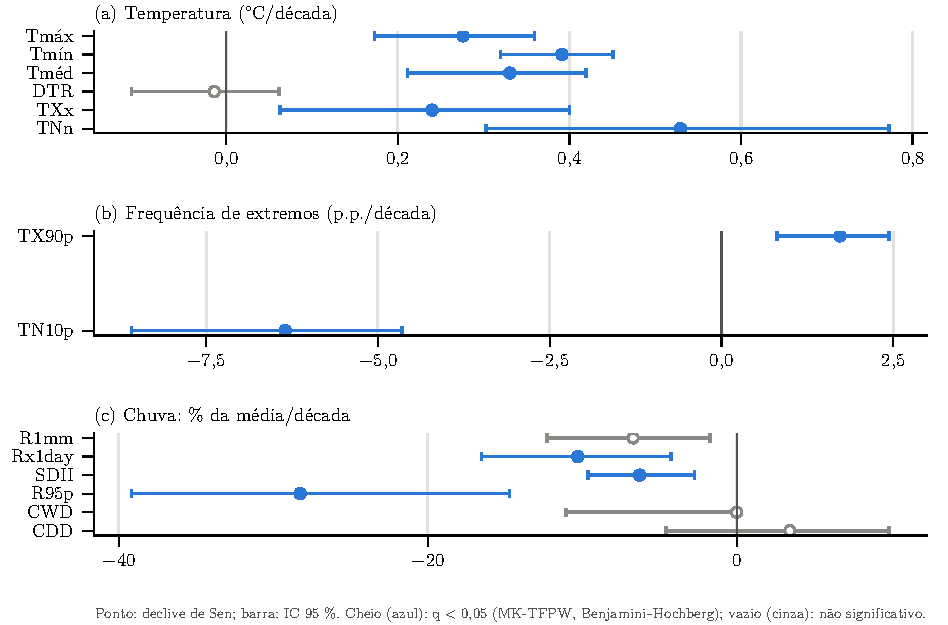
\includegraphics[width=\textwidth]{figuras/fig09_tendencias.pdf}
  \caption{Tendências por década (declive de Sen e IC de 95\,\%). Os índices de chuva estão
  em percentual da média da série.}
  \label{fig:tend}
\end{figure}

\paragraph{Distribuição da temperatura.} A regressão quantílica (\cref{fig:quant}) indica
aquecimento em toda a distribuição. A Tmín subiu \QRTminQumzero{}, \QRTminQcincozero{} e
\QRTminQnovezero{}~°C por década nos quantis 0,1, 0,5 e 0,9, e a Tmáx subiu \QRTmaxQumzero{},
\QRTmaxQcincozero{} e \QRTmaxQnovezero{}~°C. Os intervalos se sobrepõem, então não há evidência
clara de aquecimento desigual entre os quantis; todos excluem zero.

\begin{figure}[htbp]
  \centering
  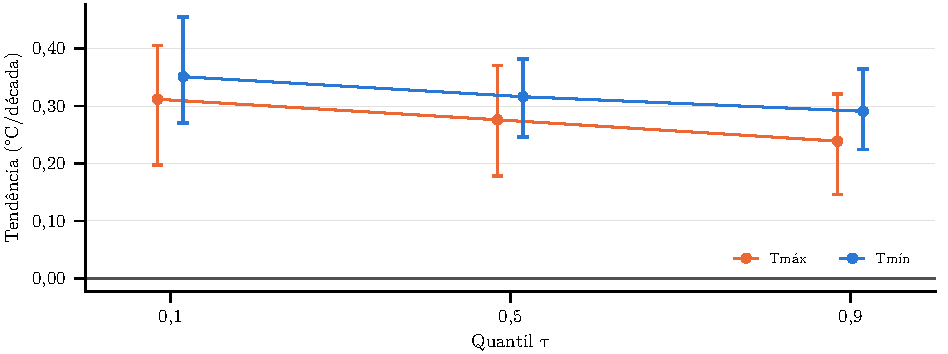
\includegraphics[width=\textwidth]{figuras/fig11_quantilica.pdf}
  \caption{Tendência por quantil da temperatura diária (regressão quantílica com controle
  sazonal; IC de 95\,\% por bootstrap em blocos anuais).}
  \label{fig:quant}
\end{figure}

% ============================================================================= discussão
\section{Discussão}\label{sec:discussao}

\paragraph{O regime mudou.} O resultado mais firme deste trabalho é que Petrolina ficou mais seca
e mais quente desde a década de 1960. A chuva anual caiu \SenChuva{}~mm por década, com
intervalo que exclui zero com folga, e a magnitude da queda é estável entre subamostras, inclusive
com os anos chuvosos recentes e sem os anos da seca de 2011/12 a 2016/17. A detecção, porém,
depende da década de 2010: até 2010/11, a mesma queda não seria significativa. Ela não é só local: a referência formada pelas vizinhas cai
\SenReferencia{}~mm por década, e \NAnaNegSig{} de \NPostosAna{} pluviômetros independentes da ANA
confirmam a queda. Contra a referência do INMET, a parte exclusiva da \Est{} coincide, com
significância marginal, com a instalação da estação automática em \QuebraQ{}; mas o pluviômetro
independente mais próximo, a \DistJuazeiro{}~km, reproduz a tendência da \Est{} nos mesmos anos e
não mostra mudança relativa nessa data. Uma contribuição instrumental não pode ser descartada, mas
não é necessária para explicar a queda. A diminuição aparece tanto nos índices de
intensidade (Rx1day, SDII, R95p) quanto no número de dias de chuva, e há indício, não confirmado
pelo teste com pré-branqueamento, de que a estação chuvosa começa mais tarde e ficou mais curta.
A forma do ciclo anual, medida pelo índice de sazonalidade e pela concentração, não mudou, e o
aumento de anos sem estação chuvosa definida não é estatisticamente significativo.

O aquecimento atinge toda a distribuição da temperatura. Na Tmín, que não tem quebra frente às
vizinhas, ele é o resultado mais firme do trabalho; na Tmáx, resiste ao corte da série em 2008 e à
correção da quebra frente a Cabrobó, embora com magnitude menor (\SenTmaxAjustada{}~°C por
década). Com noites frias ficando mais raras, a demanda
evaporativa aumenta; por isso o SPEI, que incorpora a temperatura, é uma medida mais completa do
estresse hídrico do que o SPI. Menos chuva e mais evaporação apontam na mesma direção para o
balanço hídrico local.

\paragraph{Comparação com estudos anteriores.} A queda da chuva anual e do número de dias
chuvosos, e o aquecimento com noites frias mais raras, coincidem com o padrão predominante nas
estações do Nordeste em 1961--2014 \parencite{costa2020} e com a diminuição apontada para
Petrolina em 1961--2012 \parencite{jatoba2017}. Há duas diferenças. Primeiro, a magnitude em
Petrolina é grande, mas não isolada: ela se repete nos pluviômetros independentes vizinhos, e
\textcite{carvalho2020} também encontram queda significativa em Paulo Afonso, uma das vizinhas
da referência regional. Segundo, \textcite{costa2020} relatam aumento dos eventos acima dos
percentis 95 e 99 em muitas estações, enquanto aqui o R95p e o Rx1day diminuem. Em Petrolina, a
queda atinge também a cauda úmida, e não só a frequência de chuva.

\paragraph{A seca de 2011/12 a 2016/17 nesse contexto.} A seca iniciada em 2011/12 é descrita
como a mais severa e prolongada do semiárido desde 1981, num período em que a área afetada por
seca mostra tendência de aumento \parencite{brito2018}; ela também é destacada como excepcional
por \textcite{marengo2017} e \textcite{cunha2019}. Em Petrolina, ela corresponde à sequência de
anos hidrológicos de 2011/12 a 2016/17: os três anos mais secos desde 1963 caem nesse período, e
o evento de SPI-12 que inclui 2012/13 é o mais severo do registro. A tendência ajuda a entender
essa sequência. Sob estacionariedade, um ano como 2012/13 teria período de retorno de algumas
décadas, conforme a distribuição; com a média recente, passa à ordem de uma década. Os anos secos consecutivos também são compatíveis com a queda da média sozinha, sem
persistência adicional de um ano para o outro.

\paragraph{O que os dados não conseguem dizer.} Esses números de período de retorno são ordens
de grandeza, e o cenário com inclinação regional (\TRegionalMedia{} anos em 2025) deve ser lido
lado a lado com o principal. A conclusão não estacionária depende de uma tendência log-linear ao
longo de seis décadas e de como a variabilidade acompanha a queda da média. Supor coeficiente de
variação constante leva a \TNSGamma{} anos na Gamma, mas essa hipótese é rejeitada pelos dados;
com ela relaxada, as quatro famílias dão de \TNSVarMin{} a \TNSVarMax{} anos. A média por pesos de
Akaike incorpora essa incerteza, mas só entre as candidatas consideradas. Com uma estação, não é possível separar persistência de tendência. As correlações com o
ENSO e com o gradiente do Atlântico têm o sinal esperado, não são significativas e não dependem da
tendência. Isso não contradiz o papel conhecido desses modos \parencite{hastenrath1977,moura1981}:
reflete o tamanho da amostra, com \NFaseNino{} a \NFaseNeutro{} anos por fase do ENSO. Responder
a essas perguntas com mais poder exige mais estações ou dados em grade, e não modelos mais
complexos aplicados à mesma série.

% ============================================================================= limitações
\section{Limitações}\label{sec:limitacoes}

\begin{enumerate}
  \item \textbf{Tamanho da amostra.} Com \NanosValidos{} anos válidos, os intervalos para $T$
  abrangem uma ordem de grandeza. Para o evento plurianual E3 há um único evento dessa magnitude.
  \item \textbf{Seleção do evento.} 2012/13 foi escolhido por ser extremo e está na amostra de
  ajuste. $T$ descreve a frequência de anos abaixo do limiar, e não a raridade daquele ano em
  particular.
  \item \textbf{Homogeneidade da chuva.} A queda da chuva na \Est{} é regional, mas pode ter
  também uma parte local: a razão com a referência do INMET varia \SenQ{}\,\% por década, com indício marginal
  de quebra após \QuebraQ{}. Os pluviômetros da ANA não confirmam essa quebra de forma consistente
  (o mais próximo não a mostra; dois mais distantes sugerem um excesso local), de modo que não
  sabemos se o excedente é climático ou instrumental. O cenário com inclinação regional
  (\cref{tab:retorno,tab:prob}) delimita esse efeito.
  \item \textbf{Homogeneidade da temperatura.} A Tmáx anterior a 1971 difere das vizinhas e foi
  excluída. No período analisado, \NquebrasTemp{} dos \NtestesTemp{} testes contra as vizinhas
  indicam quebra, ambos na Tmáx, e Tmáx e Tmín mostram indício de quebra frente à A307. Não
  homogeneizamos as séries: com duas vizinhas, também elas sujeitas a quebras, não é possível
  atribuir cada salto a uma estação. As sensibilidades mostram que o aquecimento da Tmáx
  persiste, mas sua magnitude fica entre cerca de \SenTmaxAjustada{} e \SenTmaxDesdeSetentaCinco{}~°C
  por década conforme a hipótese.
  \item \textbf{Forma da distribuição.} No caso não estacionário, a candidata de menor AIC é a
  normal, que tem suporte em valores negativos; isso não afeta a cauda em torno de 151~mm, mas a
  torna inadequada para valores muito baixos. A Gamma com coeficiente de variação constante tem
  cauda seca mais fina que a dos dados ($T$ empírico \TEmpiricoDozeTreze{} contra \TGamma{} anos
  na Gamma estacionária), e essa hipótese é rejeitada no caso não estacionário. Ainda assim, os
  modelos bayesianos e os estados sem tendência da persistência e das teleconexões usam a Gamma
  com forma fixa.
  \item \textbf{Período efetivo.} A chuva é analisada até \UltimoAnoValido{}. Os anos chuvosos
  \AnosFCASete{} ficam fora pelo critério de completude; incluí-los atenua a tendência, de modo
  que a exclusão favorece o resultado principal.
  \item \textbf{Forma da tendência.} O modelo não estacionário supõe tendência log-linear. Ele não
  diz por que a chuva caiu. Os valores para 2025 e a continuidade da tendência são extrapolações.
  \item \textbf{Teleconexões.} Não detectamos efeito do ENSO nem do gradiente do Atlântico; com
  uma estação e \NanosValidos{} anos, o poder para isso é baixo.
  \item \textbf{Representatividade espacial.} Os resultados são de um ponto, verificados com
  \NPostosAna{} pluviômetros independentes num raio de cerca de 50~km. Os períodos de retorno e
  os demais índices não foram calculados para esses postos, e dados em grade
  \parencite{xavier2016,funk2015} permitiriam estender a análise à região.
  \item \textbf{Linha de base externa.} As normais climatológicas oficiais do INMET para
  1991--2020 não foram comparadas; usamos a normal calculada da própria estação. A comparação
  com a climatologia de Bebedouro \parencite{teixeira2010} é só de ordem de grandeza, porque os
  anos usados nas duas médias não coincidem.
  \item \textbf{Métodos.} Hargreaves--Samani é uma aproximação da ETo, e Penman--Monteith com
  radiação estimada pela insolação seria uma verificação natural. Os índices TX90p e TN10p não
  usam a correção de \textcite{zhang2005}. A decomposição STL preenche lacunas mensais com a
  climatologia e é apenas descritiva; não ajustamos um modelo aditivo generalizado.
\end{enumerate}

% ============================================================================= conclusões
\section{Conclusões}\label{sec:conclusoes}

\begin{enumerate}
  \item A chuva anual em Petrolina caiu \SenChuva{}~mm por década
  \IC{\SenChuvaICinf}{\SenChuvaICsup} desde a década de 1960. A queda é compartilhada pelas
  estações vizinhas do INMET, com magnitude menor (\SenReferencia{}~mm por década), e confirmada
  por pluviômetros independentes da ANA; o mais próximo reproduz a tendência nos mesmos anos. Ela
  envolve tanto a intensidade quanto o número de dias chuvosos.
  \item As temperaturas mínima e máxima subiram \SenTmin{} e \SenTmax{}~°C por década, de forma
  consistente em toda a distribuição. A Tmín não tem quebra frente às vizinhas; na Tmáx, a
  correção de uma possível quebra reduz a tendência para \SenTmaxAjustada{}~°C por década, sem
  eliminá-la.
  \item O ano hidrológico mais seco desde 1963 foi \AnoMinimo{}. 2012/13 foi o
  \RankDozeTreze{}º, praticamente empatado com \RankAnotres{}, e os três primeiros estão na
  sequência seca de 2011/12 a 2016/17.
  \item Com a queda da chuva, um ano tão seco quanto 2012/13 passa de um período de retorno da
  ordem de \TMediaAkaikeB{} anos \IC{\TMediaAkaikeBICinf}{\TMediaAkaikeBICsup}, sob
  estacionariedade, para \TNSMediaUlt{} anos \IC{\TNSMediaUltICinf}{\TNSMediaUltICsup} com a
  média do último ano observado (\TRegionalMedia{} anos em 2025 com a inclinação regional). O
  valor é estável entre as distribuições quando a variabilidade não é forçada a cair junto com
  a média (\TNSVarMin{} a \TNSVarMax{} anos), os intervalos cobrem
  uma ordem de grandeza, e esses números indicam escala, não valores precisos.
  \item Os dados não separam a persistência de anos secos da tendência nem detectam a influência
  do ENSO; a sequência de 2011/12 a 2016/17 é compatível com a queda da média sozinha.
\end{enumerate}

% ============================================================================= disponibilidade
\section*{Disponibilidade de dados e código}
Os dados brutos são públicos (INMET/BDMEP, ANA/Hidroweb e NOAA PSL); a chuva dos postos da ANA
é baixada por \texttt{scripts/baixa\_ana.jl}. O código Julia, com testes unitários, e
o script que regenera todas as figuras e todos os números deste texto (\texttt{scripts/paper.jl},
que escreve \texttt{paper/resultados.tex}), além de uma verificação independente em Python
(\texttt{scripts/verifica.py}) que recalcula os números centrais a partir dos dados brutos, estão em \url{https://github.com/dantebertuzzi/meteo} e
no depósito do Zenodo deste trabalho (DOI a ser atribuído no depósito). O código está sob licença
MIT e o texto sob CC-BY 4.0.

\printbibliography[title={Referências}]

\end{document}
